\documentclass[a4paper, 12pt]{article}
\usepackage[english]{babel}
\usepackage[a4paper,left=2.5cm, right=2.0cm, top=2.5cm, bottom=2.5cm]{geometry}
\usepackage[utf8]{inputenc}
\usepackage{setspace}
\usepackage{url}
\usepackage{hyperref}
\usepackage{longtable}
\usepackage{lscape}
\usepackage[final]{pdfpages}
\usepackage{graphicx}
\usepackage{colortbl}
\usepackage{multirow}
\usepackage{listings}
\usepackage{subfigure}
\usepackage{graphicx}
\usepackage{verbatim}
\usepackage{amsmath}
\usepackage[nottoc,notlot,notlof]{tocbibind}

\newcommand{\argmax}{\operatornamewithlimits{argmax}}
\newcommand\todo[1]{\textcolor{red}{#1}}

\begin{document}
%This file will subsume all of the individual chapters of the project report


%\setstretch{1.50}
\pagestyle{empty}

\begin{center} Project Report \end{center}
\hspace{1cm}
\begin{center} Softwareproject: \end{center}
\begin{center}Spoken Dialog Systems for Elevator Control \end{center}
\begin{center} Universität des Saarlandes \end{center}
\begin{center} Department 4.7 Computational Linguistics and Phonetics \end{center}
\begin{center} Computerlinguistik, B.Sc./M.Sc. \end{center}
\begin{center} Summer term 2015 \end{center} 

\hspace{1cm}
\begin{center}Instructors: Ingmar Steiner, Asad Sayeed, Arif Khan \end{center}

\begin{center} Participants: Anne-Julia Hoffmann, Boyuan Deng, Laura Faust \end{center}


\pagestyle{plain}
\setcounter{page}{1}
\tableofcontents
\cleardoublepage
%please put in the files you wrote in the corresponding order and space by
%using \input{filename} so that we can compile the entire project report as one

\section{EllaVator}

The software project in the summer 2015 was started with the goal to revive the speaking elevator in building C4.7 
of Saarland University. It was named as "EllaVator" and for the rest of this report the name "EllaVator" will be used
to refer to the speaking elevator. The main purpose of the project was to renew the old hardware that is currently
in use, improve the overall efficiency of the elevator, update/replace the software components with open source software and
release/publish the code for free, like on github.
\newline
The elevator currently in use was installed in the year 2000, by the
computational linguistic department of Saarland University. The software
project was named "Sprachsteuerung im Aufzug". \footnote {"Voice commands in the elevator"}
The result of this project was an interdisciplinary work with the department of informatics, phonology and computational linguistics, the outcome was an elevator that can be controlled haptically by pressing buttons and also with voice command. ~\cite{SprachsteuerungimAufzug} \newline

Since then, the elevator has been in normal use for transporting people, but it also serves to introduce guests and students to one of the many fields of the application for computational linguistic;
To show them the possibilities of such an application as well as its limits. \newline
\subsection{Previous implementation}
\todo{re write this paragraph as: Issues with previous implemenation}\\
\todo{some points: Hang up unexpectedly, wrong floors entry, wrong language recognition, asking for input repeatedly}\\
\todo{some points: Old hardware, Had to be rebooted frequently}\\
The software project for the speaking elevator had since then been repeated to give students the opportunity 
of experiencing the procedure of working together on a real application while trying to further develop the speaking elevator.
In summer 2015, it was decided to work on the software as well as to replace part of the hardware.
While the hardware used inside the elevator was not touched, the computer which is connected to the elevator and runs the software being used for the voice control of the elevator was exchanged.
The hardware used before was outdated and was causing problems which is why it was decided that it should be replaced. \newline

\subsection{Our implementation}
The result of the software project "speaking elevator" of the summer term 2015
thus is not a new iteration of the application running on the elevator, but the
work done can be used with new hardware provided.
The system developed by the participants of this project runs on any computer.
If it were to be connected to the elevator it would merely have to be tested inside the elevator and adjusted to the specific conditions of reverberation and movement of the elevator. \newline

In the following, there will be given an introduction to the components of the elevator control in section  ~\ref{sec:Components_of_elevator_control} , chapter ~\ref{sec:General_thoughts} will present some basic ideas that were discussed before starting the implementation of the system.
In section ~\ref{sec:Dialog_manager} a selection of currently popular dialogue managers, as well as an introduction to the OpenDial, the dialogue manager used for the project will be given.
Mary TTS, the text to speech system that was used is presented in chapter ~\ref{sec:Speech_Synthesis}. \newline
In the sections which follow, information about the hardware used is provided.
With section ~\ref{sec:Rasberry_Pi} presenting the Raspberry PI used and section ~\ref{sec:Serial_control_of_the_elevator} the serial control of the elevator.
Section ~\ref{sec:Development_tools} contains information about the tools used for the development of the project, which are Gradle, GitHub and Travis.
The section Testing ~\ref{sec:Testing} presents the methods used to automatically test the system.
The final chapter ~\ref{sec:Installation_instructions} provides installation instruction for running the project "EllaVator".

\newpage
\section{Components of elevator control}
\label{sec:Components_of_elevator_control}

\subsection{Automatic speech recognition}
Speech recognition is a complex technology which involves many fields, such as probability theory, machine learning, statistical natural language processing and speech processing. However, the architecture of a modern speech recognizer can be broadly divided into two main components namely the Acoustic Model (AM) and the Language Model (LM). The decoder uses these two components and produces the text output of the extracted input features as shown in Figure~\ref{fig:asr_component1}.
\begin{figure}[ht]
\centering
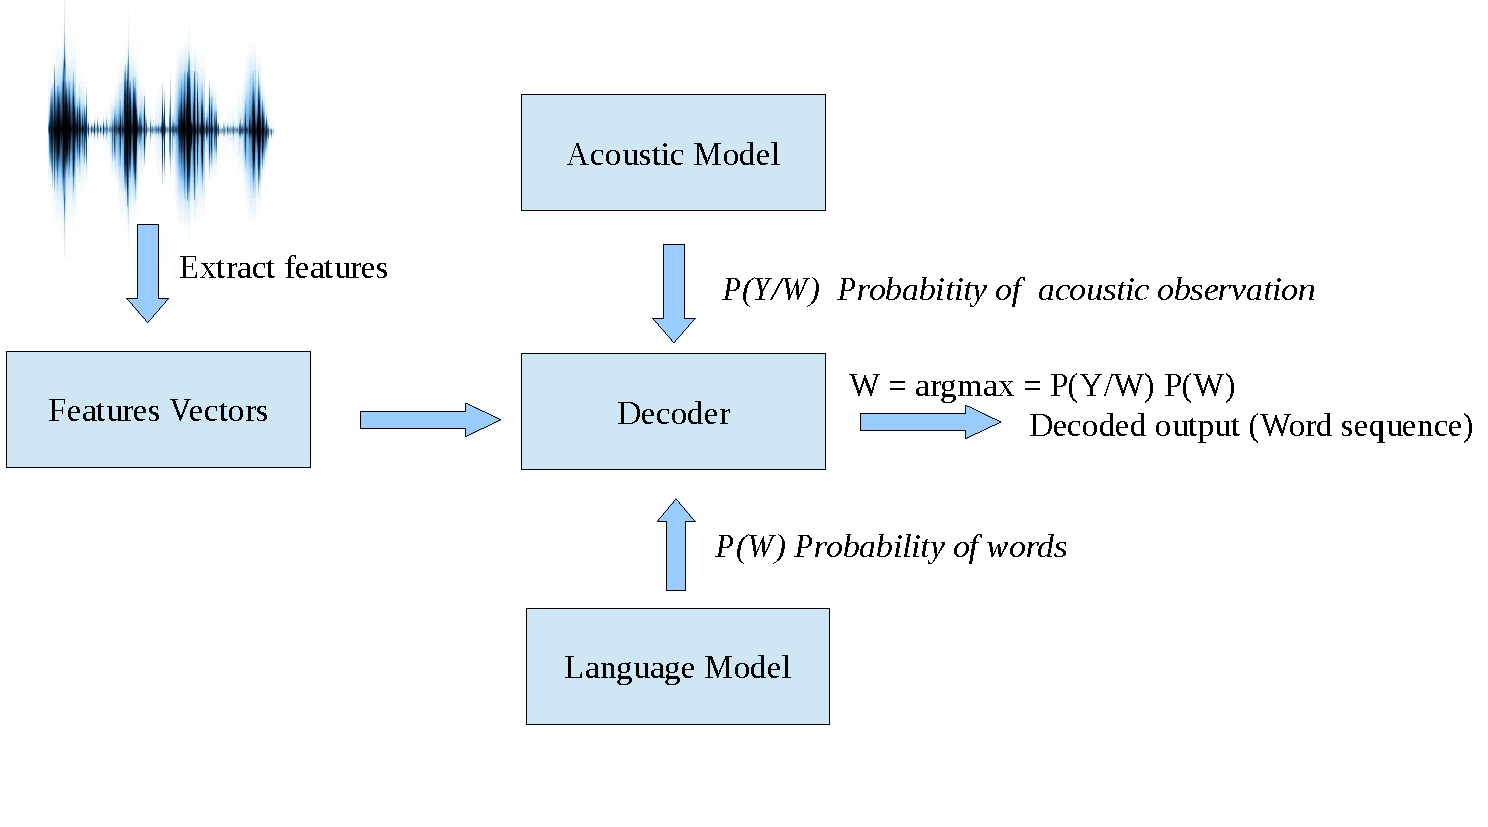
\includegraphics[width=\textwidth]{ASR_Component1.pdf}
\vspace{-1.2cm}
\caption{\textit{Basic components of speech recognition system.}}
\label{fig:asr_component1}
\end{figure}


If an utterance is represented as a sequence of words, $W$ = $w_1$, $w_2$, $w_3$, \dots \dots, $w_N$, then the decoder will try to find the most probable word sequence $\hat{W}$, given the sequence of acoustic vectors, $Y$ = $y_1$, $y_2$, \dots \dots, $y_T$. Using Byes rule, the probability of a word given an observation $P(W/Y)$ can be found as:
\begin{equation}
\label{equ:bayes_rule}
\hat{W} = \argmax P(W/Y) = \argmax\frac{P(W)P(Y/W)}{P(Y)}.
\end{equation}
In this equation, the word sequence $\hat{W}$ must be found, as the one that maximizes the product of $P(W)$ and $P(Y/W)$, where $P(W)$ is the prior probability which comes from the language model and $P(Y/W)$ is the probability of vector sequence $Y$ given some word sequence $W$, which is known from the acoustic model. $P(Y)$ is ignored, as it is a constant for all possible word sequences. Below each of the component is explained in more detail.
\subsubsection{Acoustic modeling}
The performance of the speech recognition systems mostly depends on a good acoustic model. Acoustic modeling for speech recognition refers to the process of how one can statistically represent the features vectors sequences, which are computed from the continuous speech. Since it is difficult to have frequent number of each word in the training data to accumulate acoustic statistics for that word, each word is represented into smaller units of speech called the phonemes. This is usually called the  "pronunciation modeling". In modern speech recognition systems, approximately 39-45 phonemes are used, which are combined to form all possible words in English. To model the acoustic features, Hidden Markov Model (HMM)~\cite{hmm_for_SR} are used.

\subsubsection{Language modeling}
The language modeling (LM) specifies what sequence of words to expect in the speech given the previous word or sequence of $N$ words. In equation~\ref{equ:bayes_rule}, the term $P(W)$ represents the language model. Many techniques have been used to estimate the probability, $P(W)$. Two of the most important techniques are mentioned below.
\subsubsection*{Formal language models}
\label{sec:gramar_based_lm}
The formal or grammar based language model is composed of a grammar and a parsing algorithm. The grammar specifies allowable structure of a language and the parsing specifies the analysis method to check if rules of the grammar are respected. For small size recognition task, often the grammar based language model is a good solution.
\subsubsection*{Probabilistic language models}
\label{sec:prob_lang_model}
The probabilistic language models assigns probabilities to words $\textit{W}_k$ based on preceding words $\textit{W}_k^{k-1} = \textit{w}_1 , \cdots \cdot,\textit{w}_{k-1}$  from a training corpus. The most commonly used language model from this category are the $N$-gram language models, where $N$ means number of preceding words to be considered. Some variations are \textit{unigrams}, \textit{bigrams} and \textit{trigrams}.

For \textit{trigrams}, where \textit{N=3} we can calculate the probability as:
\begin{equation}
  \hat{P}(w_k | w_{k-1},w_{k-2}) = \frac{c(w_{k-2},w_{k-1},w_k)}{n(w_{k-2},w_{k-1})}
\end{equation}
where $c(w_{k-2},w_{k-1},w_k)$, specifies the number of times, the words $w_{k-2},w_{k-1}$ and $w_k$ comes together and $n(w_{k-2},w_{k-1})$, specifies the number of times the words $(w_{k-2},w_{k-1})$ occurs together.

\subsection{Language model for the elevator}
For the elevator, a grammar-based language model was used, since the vocabulary size is small and the possible commands to the elevator can be modelled by the grammar.
It consists of a set of two simple grammars, one in German and one in English, in the JSGF format\footnote{http://www.w3.org/TR/jsgf/} that is usable with Sphinx.


\subsection{Dictionaries for the elevator domain}
Two dictionaries, one in German and one in English, were created to generate representations for the Sphinx speech recognition and speech synthesis and to connect with the JSGF grammar.
They both contain just under 200 words with their respective phonetic transcriptions.
The vocabulary is made up of the names of the people working in building C7.4, as well as numbers, room names such as "laboratory" or "restrooms" and all other words relevant to the limited elevator domain.
Each of the words is followed by its phonetic transcription in the ARPAbet phoneme set.
The ARPAbet maps each of its currently 39 phonemes to one single or a pair of ASCII characters.
The English dictionary is based on the CMU Pronouncing Dictionary\footnote{http://www.speech.cs.cmu.edu/cgi-bin/cmudict\#lookup}, an open-source  machine-readable pronunciation dictionary for North American English.
Words that could not be found in the existing CMU dictionary, which was mainly the case for proper nouns, were entered into the LOGIOS lexicon tool.\footnote{http://www.speech.cs.cmu.edu/tools/lextool.html}


The German dictionary is based on the voxforge German CMU dictionary which can be found via sourceforge.%
\footnote{http://sourceforge.net/projects/cmusphinx/?source=typ\_redirect}








\subsection{Reverberation recordings in the elevator}

\begin{figure}
\center{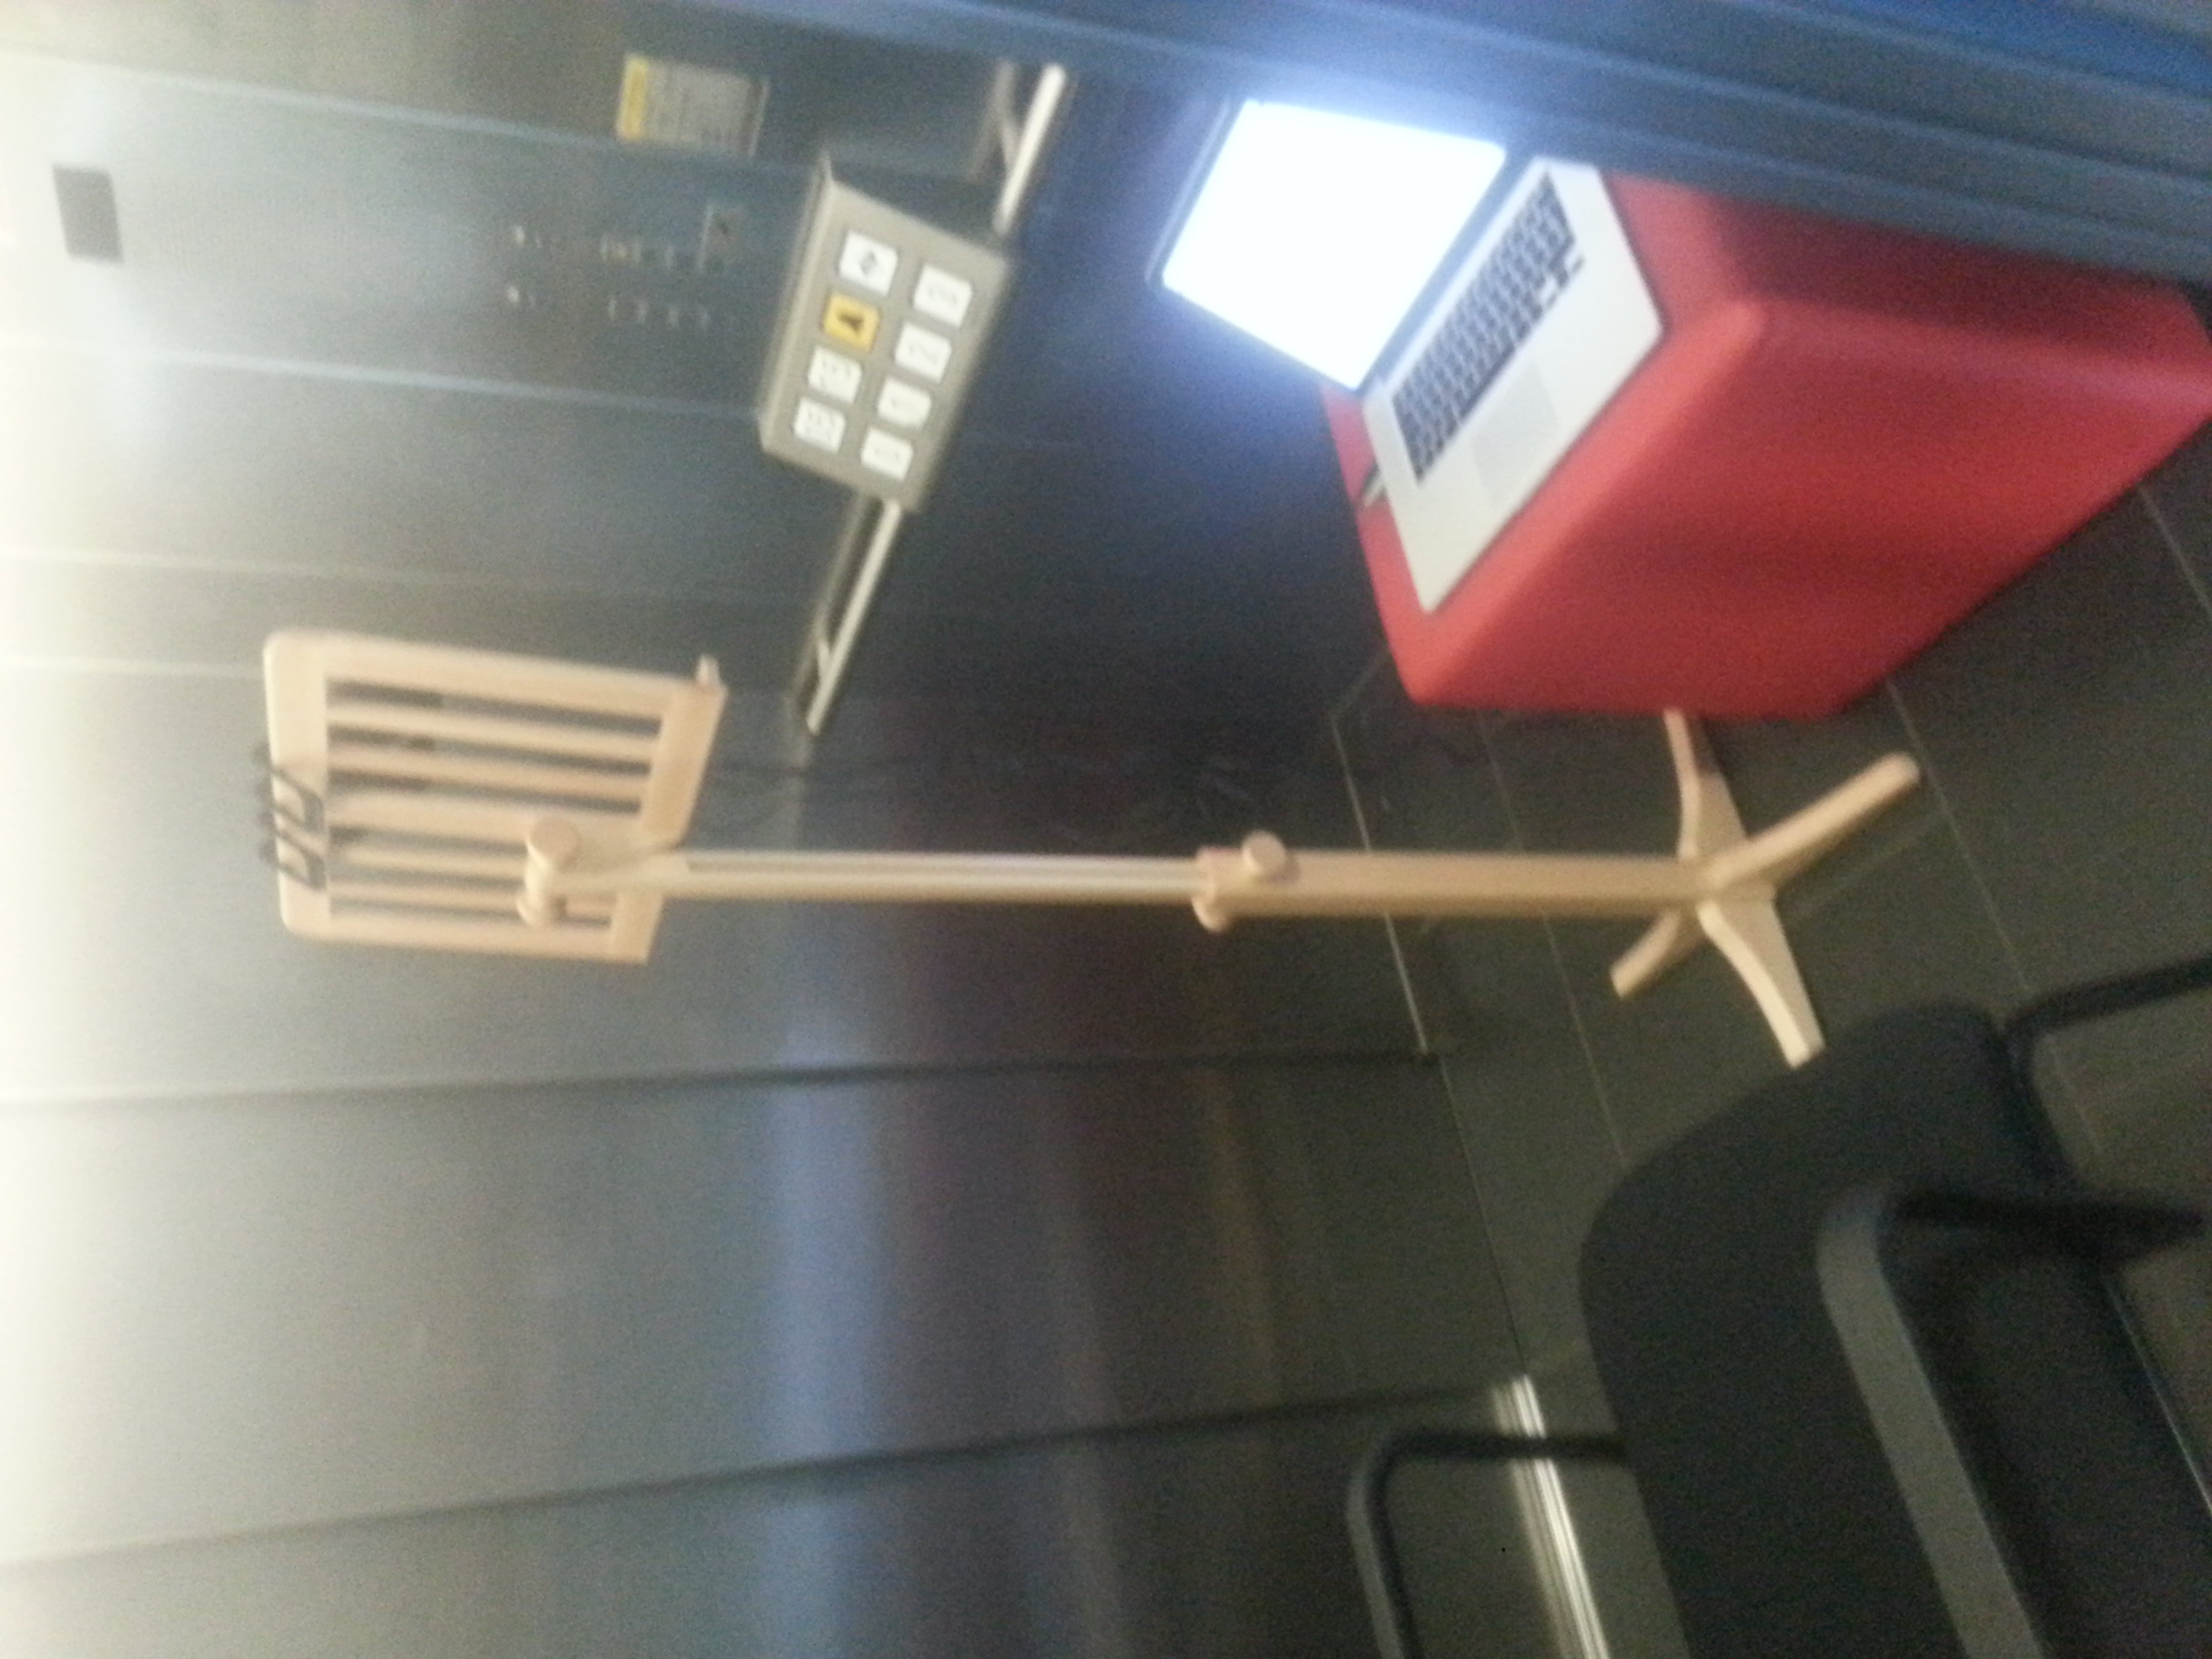
\includegraphics[scale=0.10, angle=-90]{setup_reverberation_rec.jpg}}
\caption{Recordings setup.}
\label{fig:recordingsetup}
\end{figure}


To train the acoustic model for the elevator, recordings of elevator-specific commands and phonetically balanced sentences in both English and German were made.
Lists one and two  of the Harvard sentences\footnote{http://www.cs.columbia.edu/~hgs/audio/harvard.html} were used as phonetically balanced sentences in English and twenty sentences taken from BITS\footnote{http://www.bas.uni-muenchen.de/forschung/Bas/BasBITSUSTABLE} were used for German.
The full list of sentences which have been used can be found in the appendix \ref{prompts}.
The sentences were read by all of the participants and recorded in a sound proof studio.
This resulted in recordings of English sentences spoken by non-natives and German sentences spoken by natives and by non-natives.


The commands that are spoken inside the elevator, are taken via a cable to the system where they are then processed. But during this process some distortion is produced. This distortion might be caused by cable or some other external factor. To account for this noise of the elevator and the sound of the opening/closing of doors and other noises from outside of the elevator, further recordings were made via the elevator's built-in microphone. The setup used for this can be seen in Figure \ref{fig:recordingsetup}.

It consisted of two loudspeakers positioned on a music stand at the height of approximately 150cm, at a distance of approximately 20cm from the elevator's microphone.
The recordings made in the lab were played through the loudspeakers and recorded with Praat via the elevator's microphone.
While the recordings were being played, the elevator was moved between the floors, its doors were opened and closed and kept stationary with its doors opened and closed on different floors.

\newpage
\section{General thoughts}
\label{sec:General_thoughts}
Before actually starting to work on the dialogue itself, it was first decided how a dialogue with the EllaVator should look like. \\

The Participants came up with the following model: \\


\begin{figure} [ht]
  \center{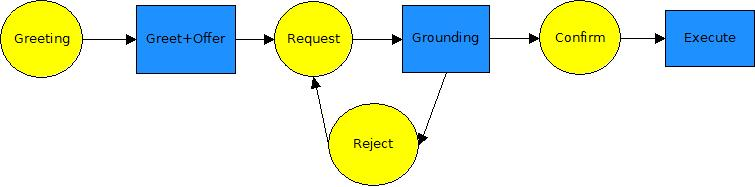
\includegraphics[scale=0.8, angle=0]{Dialogue_model.jpeg}}
  \caption{A model for the Dialogue}
  \label{fig: Dialogue flow}
\end{figure}

In the figure shown above commands from the user are marked in yellow, the answers from the EllaVator are marked in blue.
Here is a table giving example sentences for the states indicated by the figure above: \\


\begin{tabular}{|ll|}
  \hline
  Greeting & The user greets the elevator with a keyword \\
    & and thus activates the system.  \\
  Greet + Offer & Hello, how can I help you? \\
  Request & Take me to floor/room XY/ Name\_of\_a\_person \\
  Grounding/Clarify & You'd like to be taken to ...?\\
   & I didn't get it, could you repeat that? \\
  Confirm & Yes \\
  Reject & No \\
  Execute & Okay I shall now take you to ... \\
   & *here the elevator should also start the action of moving* \\
  \hline
\end{tabular}
\newline
Of course the actual system should be able to understand a variety of sentences and maybe alternate the answers but the dialogue itself can be kept as simple as it is shown in the graph.  \\

Although the idea of including some chatting with the user or small Easter eggs was appealing, it has not yet been implemented.
Measurements were made on how much time the average user spends in the elevator to determine how much time there is for the dialogue.
On average the elevator needed 40 seconds to go from the ground floor to the top and 21 seconds for going down. Opening the Doors takes 4 seconds, closing them 5.5 seconds.
With this in mind it was decided that the dialogue should be kept as simple as possible as one of the reasons for everyone using the elevator is to be faster compared to taking the stairs.
One point was that maybe the likelihood of people using the speech interface would be lower if too much time was spend on such interactions.\\

Instead, it was discussed whether the dialogue design should enable the user to merge the state "Greet" with the state "Request" which would allow for the user to both activate the elevator and also enter where they would like to be taken to.
This would skip one state from the user as well as one step from the elevator.
It was also being discussed that depending on the confidence of the user input the state "Grounding" could also be skipped have a shorter dialogue.\\

The system was then implemented as is described in the graph above, with the options noted above still kept in mind, but having them rather as a option to adapt the system to the specific conditions within an elevator.\\

Another thought that was put aside to work on after the system has been tested in the actual environment was that it might be the case that more than one person enters the elevator and that these people might have different destinations.
Of course it would be possible to just run the dialogue with one person, take them to their destination and then run the dialogue again with the next person.
This approach might however be inconvenient.
It might be more natural to enable the system to take more then one request.\\

Another problem that arose when thinking about the scenario of more than one person entering the elevator, was that they might not share the same language.
For the project EllaVator an English as well as a German version of the system is provided.
So the problem was not only to allow for multiple inputs but also for multiple inputs in different languages.\\
\newline

\textbf{
  \begin{center}Switching between languages... \\
    \underline{Our thoughts on this are collected in ticket 80}\\
    @Naska \\
    @Laura \\
    does one of you feel like writing a little about this issue?
\end{center}}

\newpage
\section{Dialog manager}
\label{sec:Dialog_manager}
The dialog manager is responsible for keeping track of the conversation and deciding the next move of the system for each input. The domain of our project is fairly limited. Most conversational situations consist of the user naming a location and the machine taking the action of moving to that location and reassuring the user that it had understood the command. This can described by deterministic If...then... statements. A dialog manager that models the conversation flow as an deterministic FSA is well-suited for our needs.
When choosing the dialog manager for our project, we considered the following factors: It had to be open source, preferably Java and well documented.
We were also looking for code that was actively maintained.
We reviewed a few potential contenders:
\begin{itemize}
\item[IrisTK] \hfill \\
IrisTK is a sophisticated dialog manager. The main focus of this dialog manager is multimodality i.e it can integrate input from multiple sensory inputs, for example speech and vision. The multimodal nature of this manager adds a lot of functionality which we would not have used, so we decided not to use it.
\item[InproTK] \hfill \\
The most exciting asset of this dialog manager was incremental processing.
The code is well maintained and actively developed.
However, we failed to build a demo that uses incremental features due to the lack of documentation so we dropped this option.
\item[OpenDial] \hfill \\
OpenDial is probably the most popular open source dialog manager.
After successfully implementing a short domain-relevant demo, we opted for this dialog manager.
For more detailed description, see section ~\ref{sec:opendial}.
\end{itemize}

\subsection{OpenDial}
\label{sec:opendial}
Opendial was used to implement not only the dialogue manager,  but also the main class: the dialogue system.
Opendial handles the whole dialogue system, which consists of the automatic speech recognition (ASR), the dialogue manager and the text-to-speech (TTS) system.
A collection fo plugins was used to connect external plugins to the dialogue system: Sphinx 4 ~\cite{Walker:2004:SFO:1698193} for ASR and MaryTTS ~\cite{marytts} for text to speech.
This means that Opendial takes care of updating the dialogue manager's variables on speech input (coming from the ASR module), and forwarding the dialogue manager's output to the text to speech module.
The main component that has to be implemented for the dialogue manager is the domain file. \\
\indent Like most dialogue managers Opendial also consists of three different components which interact to create a dialogue.

The first component is responsible for the recognition of language.
In OpenDial this component is called ”Natural Language Understanding model (NLU)”.
The output of the first process is passed on to the next component which checks if there was an instruction given which action should be be performed upon that input.
Such actions might be showing something on a GUI, starting a task or simply selecting an answer to the user's input.
In OpenDial this part is called ”Dialog Manager”.
The third and last component is called ”Natural Language Generation module (NLG)” and is basically the opposite of the NLU.
The NLU generates language from the output of the ”Dialog Manger”.
Though the component is named NLG, the output of a dialogue system is not necessarily speech, but the output is often designed so that it can be easily used to generate speech with a TTS component.
This is also the case for OpenDial.
OpenDial also offers a GUI where the dialogue (input and output) is displayed without having to use further plugins.

\subsubsection{Domain}

All of the components mentioned above are located in the so called Domain file.
A dialogue designer working with OpenDial will, in most cases just have to work on this one file.
For easier readability, it can of course be split into smaller files, which will then have to be imported into one single file.
As the complete dialogue for the elevator is rather small it was not split for the project EllaVator, but kept in one file. \newline

This file provides instructions for the system on what to do.
The user's input will be first transformed into an XML structure and then further processed.
Some systems fill this structure with semantic information.
OpenDial however basically passes variables through the components of the system.
The dialogue designer can then assigns values to those variables which will ultimately determine the flow of the dialogue.
There is a convention for the naming of the variables, they can however be named to the dialogue designers liking.
As all information is being passed through variables the correct naming is important though.
All three components have a slot ”trigger” at the very beginning of their structure.
The value given to this slot has to be the name of all variables which are to activate this component.
For example giving the component this trigger:
\textless model trigger=”a\_u” \textgreater will make it respond to all variables with the name ”a\_u”. \\


So the variables in OpenDial do not only carry the value through the system but their names also determinate which module should continue to process that variable.
The most common way to link them was described in the previous section.
Having the NLU module process the user's input, the dialogue manager process that input and then responding using the NLG module.
In case there is no further processing needed one might also decide to directly link NLU module to NLG module.
If the system should for example ask a question after having said something, it might also be possible that the dialogue designer might want to trigger the NLG twice, either linking NLU to NLG module or NLU module to the dialogue manager which again links back to the NLG module.


The Domain-file is subdivided into three parts as they each represent one components these parts are called modules.
The modules themselves are again subdivided into rules, with every rule representing one command.\\

In the following subsections, information about each component will be given.
The user-manual of Open Dial \cite{OpenDial} was used as the main source for the following subsections.
For further instructions as well as example code illustration the more advanced possibilities given by Open Dial, please see the webpage \url{http://www.opendial-toolkit.net/user-manual}.

\subsubsection{Natural Language Understanding module}

The first model to receive input is the ”Natural Language Understanding module” (NLU).
Depending whether further plug-ins are used, this module will get its input either directly from the user or from the plug-in.
OpenDial NLU component is able to work with plain text input from the user, but in the case of the Ellavator project the user shall also be able to use speech commands to operate the elevator, therefore the NLU in this project receives input from the grammar file of the Sphinx plug-in.
The grammar of the Sphinx plug-in already does part of the work, which would be usually done by the NLU alone.
There is only a very limited amount of commands which the elevator is able to execute.
Each of those can however be triggered by various expressions, as different people will use different words and structures to express themselves.
Therefore a domain-file that should be capable of doing something should have at least one rule which can be activated by at least one expression. \newline


In the example shown below there is a rule which models the command of changing a direction.
A rule consists of at least one case-expression.
A case-expression itself consists of a ”condition” and an ”effect”.
 In the ”condition”, as the name already states the dialogue designer can define under which circumstances a case-expression will match the users input.
 These conditions are connected using a logical operator.
 In most cases one would want to use the conditions ”or” as either one of those expressions should trigger the rule.
 The ”effect” will be the value passed on to the dialogue manager.
 As stated before this is done by assigning a variable of the proper name a value.
 In the case of the example below the variable is assigned the value of the function of changing to floor to the level of the given parameter.



  \textless rule\textgreater \newline
  \indent \indent \textless  case \textgreater \newline
  \indent \indent \indent \textless condition operator=”or”  \textgreater \newline\indent \indent \indent \indent \textless if var=”u\_u” value=”go to second floor” relation=”contains”/  \textgreater \newline
  \indent \indent \indent \indent \textless if var=”u\_u” value=”take me up to the second floor” \newline
  \indent \indent \indent \indent relation=”contains”/ \textgreater \newline
  \indent  \indent \indent \indent \textless if var=”u\_u” value=”second floor” relation=”contains”/ \textgreater \newline
  \indent \indent \indent \textless /condition \textgreater \newline
  \indent \indent \indent \textless effect prob=”1” \textgreater \textless set var=”a\_u” value=”Request(second)” / \textgreater \newline
  \indent \indent \indent \textless /effect \textgreater \newline
  \indent \indent \textless /case \textgreater \newline
  \indent \indent \textless case \textgreater \newline
  \indent \indent \indent \textless condition operator=”or” \textgreater \newline
  \indent \indent \indent \indent \textless if var=”u\_u” value=”go to thrid floor” relation=”contains”/ \textgreater \newline
  \indent \indent \indent \indent \textless if var=”u\_u” value=”take me up to the third floor” relation=”contains”/ \textgreater \newline
  \indent \indent \indent \indent \textless if var=”u\_u” value=”third floor” relation=”contains”/ \textgreater \newline
   \indent \indent \indent \textless /condition \textgreater \newline
   \indent \indent  \textless effect prob=”1” \textgreater \textless set var=”a\_u” value=”Request(third)” / \textgreater \newline
   \indent \indent  \textless /effect \textgreater \newline
   \indent \indent \textless /case \textgreater \newline
   \indent \textless /rule \textgreater \newline


In the example above one rule is shown.
This one rule includes two different commands.
They are gathered in one rule as they both are orders to switch a floor.
The only difference is the floor level they have.
Resulting in different parameters which are given to the function of the variable ”a\_u” in the ”effect” slot. \newline



As stated before, every user will use different words to express themselves.
To cover all possible utterances for a command is impossible.
But the dialogue designer should try to at least cover the most common ones,  to make the dialogue more natural for the user.
This part can also be done in the grammar of Sphinx.
OpenDial offers a few possibilities to do so.
The first possibility would be to simply list all the expressions as it is shown in the figure above.
But as can easily be seen in the example above, there is only a small difference between the sentences.
If one would like to cover all possible sentences by merely enlisting them the Domain file will not only get extremely huge it will also be hard to read. \newline

   \begin{tabular}{|ll|}
     \hline
      a? & The word ”a” may or may not occur in the expression .  \\
     \hline
      (a \textbar b \textbar... \textbar x) & One of the symbols written  in the brackets has to occur.\\
     \hline
      (a \textbar b \textbar... \textbar x))? & One of the symbols written in the brackets may or may not occur.  \\
     \hline
   \end{tabular}
   \newline

   This table shows the expressions which can be used to structure a the NLU. \newline \newline

   In the example used above all three user-utterances could be shortened down using the expression:
   \textless if var=”u\_u” value=”(go \textbar take me) (up to the)?  second floor” relation=”contains”/ \textgreater

   Using this expressions is therefore recommended.

   \subsubsection{Dialogue Manager}

If the variable which was assigned in the NLU module was named correctly, it should, in most cases, first be passed through the dialogue manager (DM).
In the DM, the effect of a rule is triggered. A mapping occurs which links the input provided by the NLU to another structure that will trigger a reaction of the system.
As was said in the last subchapter, values in OpenDial are saved within and passed through variables, the input from the NLU will therefore be assigned to another variable. \newline

Just like all other modules, each command in the DM is divided into rules, each of them having a condition, when they are to be activated.
Therefore, in this component the output of the NLU component will be matched against all conditions in the DM.
   As soon as one matching rule is found, that rule is triggered which sends the ”effect” of that rule.
   The effect of a rule is saved into a variable.
   If no further work, like printing information on a GUI is done, one could argue, that all the DM does is basically linking two variables, the one given in the ”condition” to the variable written in the ”effect”.
   Of course not all parameters do have to be listed.
   It is sufficient to merely put a placeholder in curly brackets to indicate that there is a parameter to be passed on. \newline


   \textless rule id=”Movement” \textgreater \newline
    \indent \indent \textless case \textgreater \newline
    \indent \indent \indent \textless condition \textgreater \newline
    \indent \indent \indent \indent \textless if var=”a\_u” value=”Request(\{x\})” / \textgreater \newline
     \indent \indent \indent \textless /condition \textgreater \newline
      \indent \indent \indent \textless effect util=”1” \textgreater \newline
       \indent \indent \indent \indent \textless set var=”a\_m” value=”floor(\{x\})” / \textgreater \newline
        \indent \indent \indent \textless /effect \textgreater \newline
        \indent \indent \textless /case \textgreater \newline
        \indent \textless /rule \textgreater \newline

The figure above shows  a rule called ”Movement” which links the users input ”Request” with any parameter to the effect of that input.
The variable with the name ”a\_m” and the value ”floor” with the input of the Request is send.
The parameter specified in the placeholder ”x” written in curly brackets.
\subsubsection{Natural Language Generation module}
The last part of the system generates the speech.
Without any further plug-ins this will be done by printing the text to the GUI.
As stated before, this component basically does the opposite of the Natural Language Understanding module.
Instead of transforming the user's input into an XML structure, the system takes the last components output, which is a variable embedded in an XML structure and transforms it back to plain text, either spoken, if plug-ins are used, or printed on the GUI, if no plug-ins are used. \newline

Each command is again given its own ”rule” and ”case” structure, in which condition and effect are included.
The effect of this rule is saved in a variable but also used as output for speech. \newline

\textless rule \textgreater \newline
\indent \indent \textless case \textgreater \newline
\indent \indent \indent \textless condition \textgreater \newline
\indent \indent \indent \indent \textless if var=”a\_m” value=”floor(\{x\})” / \textgreater \newline
\indent \indent \indent \textless /condition \textgreater \newline
\indent \indent \indent \textless effect util=”1” \textgreater \newline
\indent \indent \indent \indent \textless set var=”u\_m” value=”Okay, I will now take you to the {x} floor.” / \textgreater \newline
\indent \indent \indent \textless /effect \textgreater \newline
\indent \indent\textless /case \textgreater \newline
\indent \textless /rule \textgreater \newline

The example above shows one rule from an NLG module.
In this rule, a variable to which a function  is assigned, triggers the speech output of an acknowledgement from the system.

\section{ModuleElla - from OpenDial to the elevator}
The Java module ModuleElla serves as a connection between the OpenDial module and the elevator controller. 
It transforms the information from the dialogue manager about the movement of the elevator cabin into a digit which is then handed on to the controller. 
The class ModuleElla contains a logger and a reference to the controller to speak with the elevator via the serial port. 
To ease development there is also a graphical output of the current state.
The JFrame graphics output (line 40 and 54 to 71) creates a grid of the building's six floors to show the position of the elevator while testing the system. 
In the ModuleElla file the controller is commented out at the moment, because the system is not yet connected to the elevator, which causes it to crash. 
Because of this, the initial position of the elevator is also set to 0. 
The information about the current position of the elevator is needed for commands like "one floor up".
If it is not paused, the trigger (line 79) looks at the a_m (action variable) from the dialogue manager. 
If the variable is "Movefloor" then the correct floor is locked up and the changePosition is called. 
ChangePosition (lines 102-124) maps the variables like "zero" and "zero point five" to the floors 0 to 5.
The pushButton call to the controller is again commented out in lines 127 to 129, because the controller does not work.
The JFrame graphics are updated to the new position (line 131). 
There are also two methods for OpenDial, one for pausing it (line 145) and one to see if it is paused (line 153).


\newpage
\section{Speech synthesis}
\label{sec:Speech_Synthesis}
The final step in creating the speaking elevator "Ella" was of course to make it actually talk to the user.
For this a Text-to-Speech system (TTS) had to be used. A TTS system will read out information to the user, generating voice for the input text. TTS systems are widely used today.
For example in train stations, there are announcements informing passengers about delays or if there are changes causing a train to depart from a different platform as planned.
There are screen readers for the visual impaired, which read out the elements of a screen, as well as systems which are used by the speech impaired to communicate and speak in their stead.
One of the most famous applications is the dialogue system "Siri" (Siri inc) which has been used since 2011 on the iPhone. \newline \newline
MaryTTS ("\textbf{M}odular \textbf{A}rchitecture for \textbf{R}esearch on Speech S\textbf{Y}nthesis") was chosen as the system for the talking elevator.
Not only was it developed in cooperation with Saarland University, it also offers many advantages to other TTS and therefore seemed perfect for the task.\newline

Written in the programming language Java it was designed in a collaboration between the  "Language Technology Lab" of the DFKI \footnote{(\textbf{D}eutsches-\textbf{F}orschungszentrum für \textbf{K}ünstliche \textbf{I}ntelligenz) - The German Research Centre for Artificial Intelligence} and the department of phonetics of Saarland University.
As MaryTTS is an open Source project, the code can be read by everyone. Furthermore, everyone is allowed to change and adjust it to their needs.\newline \newline
MaryTTS is build in a "modular architecture" which means that it consists of different components, each dealing with a specific task. We will take a closer look at these in the following subchapter.
The second part of the name states the purpose Mary was developed for.
It was developed for research having a modular structure and also being a open source project makes it really easy to use Mary for any research projects on speech synthesis. \newline \newline
Mary is a multilingual TSS, featuring the languages English (British as well as American), German, Telugu, Turkish, Russian, Swedish and Italian.
Further languages might be included in the future, but can also be added by any user. \newline \newline

\subsection{Modules}

Mary is subdivided into different modules.
This allows the user to take a look at the output of each of those components.
One could also interchange small details in one component and observe the output on the complete system, as well as completely interchanging a component.
In most cases these components were not specifically designed for Mary.
It would go beyond the scope of this paper to mention all of them.
Detailed information can be found on the website \url{http://mary.dfki.de/ }.

\subsubsection*{Input}

Mary accepts different kinds of inputs, the simplest one being plain text.
But Mark-up Languages such as SABLE or SSML can also be used.
These are based on the Mark-up Language XML and are developed especially for the use in TTS.

In case of the elevator, only the output of the OpenDial dialogue manager is passed to Mary, which is plain text.
Any input given to Mary will be transformed into a "MaryXML Mark-up Skeleton".
A skeleton which already has different slots which will be filled by the system in the other modules.
If the input was already in a form of Mark-up language the keys assigned in this Mark-up Language will be kept and added to the skeleton. Some of the values however might be dropped.

\subsubsection*{Tokenizer}

The tokenizer identifies the tokens of a text. The output of this module will be sentences and words which will be marked as such.
Any token will be enclosed by "\textless t\textgreater ...\textless  t\textgreater".
These marks are however just placeholder.
Later on, further information will be saved in these slots.
Analogous a sentence is enclosed by "\textless s\textgreater ... \textless s\textgreater".
Marking a dot as a sentence might seem obvious at first, but can prove quite difficult if there are other tokens in the text which also come with a dot, but do not mark the end of a sentence, such as the dot placed after titles.

\subsubsection*{Preprocessing}

This module, also called "Text-normalisation" does only work on very specific tokens.
It is only needed for acronyms or numbers.
For acronyms, the system will have to decide whether to pronounce them as one word or spell each letter out separately.
Numbers are divided into ordinal- and cardinal numbers.

\subsubsection*{Tagger and Chunker}

This module has two different tasks to solve.
The Chunker labels the constituents in each sentence.
These are distinguished between adjective, nominal and prepositional phrase.
A statistical POS-tagger working with trigram probabilities \footnote {To assign the correct word class the tagger does not only consider the current word but also the two words which were used last, making it a total of three words.} is used in order to assign every word its proper word class.

The findings of the two components are saved within the placeholders that were created by the tokenizer.
Unfortunately this also means that some of the information given by the chunker will be lost. This would be the case for local ambiguities.


\subsubsection*{Phonemisation}

This module also describes the work of several smaller steps.
The output of this system will be the transcription of every word into phonetic transcription.
To able to do this however there still needs to be some information extracted.
One of the steps needed is called "inflection endings".
In this process, the tokens marked in the step "Preprocessing" are reviewed.
With the information given by the Chunker in the earlier steps as well as under the use of an morphologic analyser these tokens such as ordinal number can now be expanded.\newline
\indent In this step Mary will also check a dictionary specifically designed for Mary by the DFKI.
It contains information about the stem of a word as well grammatical information, which reduces the amount of data as regular words can be conjugated and inflected according to those rules.
In case there is no information found about a word in the dictionary the "letter to sound conversion" will be used.
The output of this module only contains the SAMPA transcription and a note in case a word was processed by the "Letter to sound conversion".
Information on intonation will not be seen in the output.

\subsubsection*{Prosody rules}

After the last module has assessed the intonation of a word, this module will analyse the prosody of the entire text.
The end of a sentence is a classic example for the intonation of a sentence. One of the most important aspect of prosody of a text are the pauses which have to be added to it.
These will not only be added at the end of sentences but also at the end of paragraphs or chunks within a sentence.
The work of the chunker and tagger is therefore of great importance for this module.
\newline
\indent Though not all of the information will be seen in the output of this module, every word will contain a new field called "accent" in its placeholder, where the information about the intonation of the word will be stored.

\subsubsection*{Postlexical and Phonological process}

In this step the data will be revised and everything will be put into context.
Smaller details such as glottal stops or elisions at the end of a word are being added.
After this step the skeleton which has been created at the beginning of the process is filled with the maximum of information being available to Mary.

\subsubsection*{Calculation of acoustic parameters}

This module will abandon the structure of the MaryXML structure.
Instead, the output will be a list of segments, their duration and the corresponding F0 value \footnote {The F0 value is a number describing the format 0, or the fundamental frequency of a voice and indicates the pitch.}

\subsubsection*{Synthesis}
In this final step, the values acquired in earlier steps will at last be converted into sound.
The modular architecture of Mary makes it easy to interchange the synthesis module as long as it supports the format of the output given by the previous module.
Currently MBROLA ~\cite{dutoit1996mbrola} is used in by Mary, which was selected as it creates a low distortion in the signal.

\newpage
\section{Raspberry Pi}
\label{sec:Rasberry_Pi}
To implement the project, a Raspberry Pi is used instead of a conventional computer. The Raspberry Pi is a single-board computer
developed in the United Kingdom by the Raspberry Pi Foundation. The
\textit{RPi 2 model B} shown in the Figure ~\ref{fig:Pi2} was used.
\begin{figure}[ht]
\centering
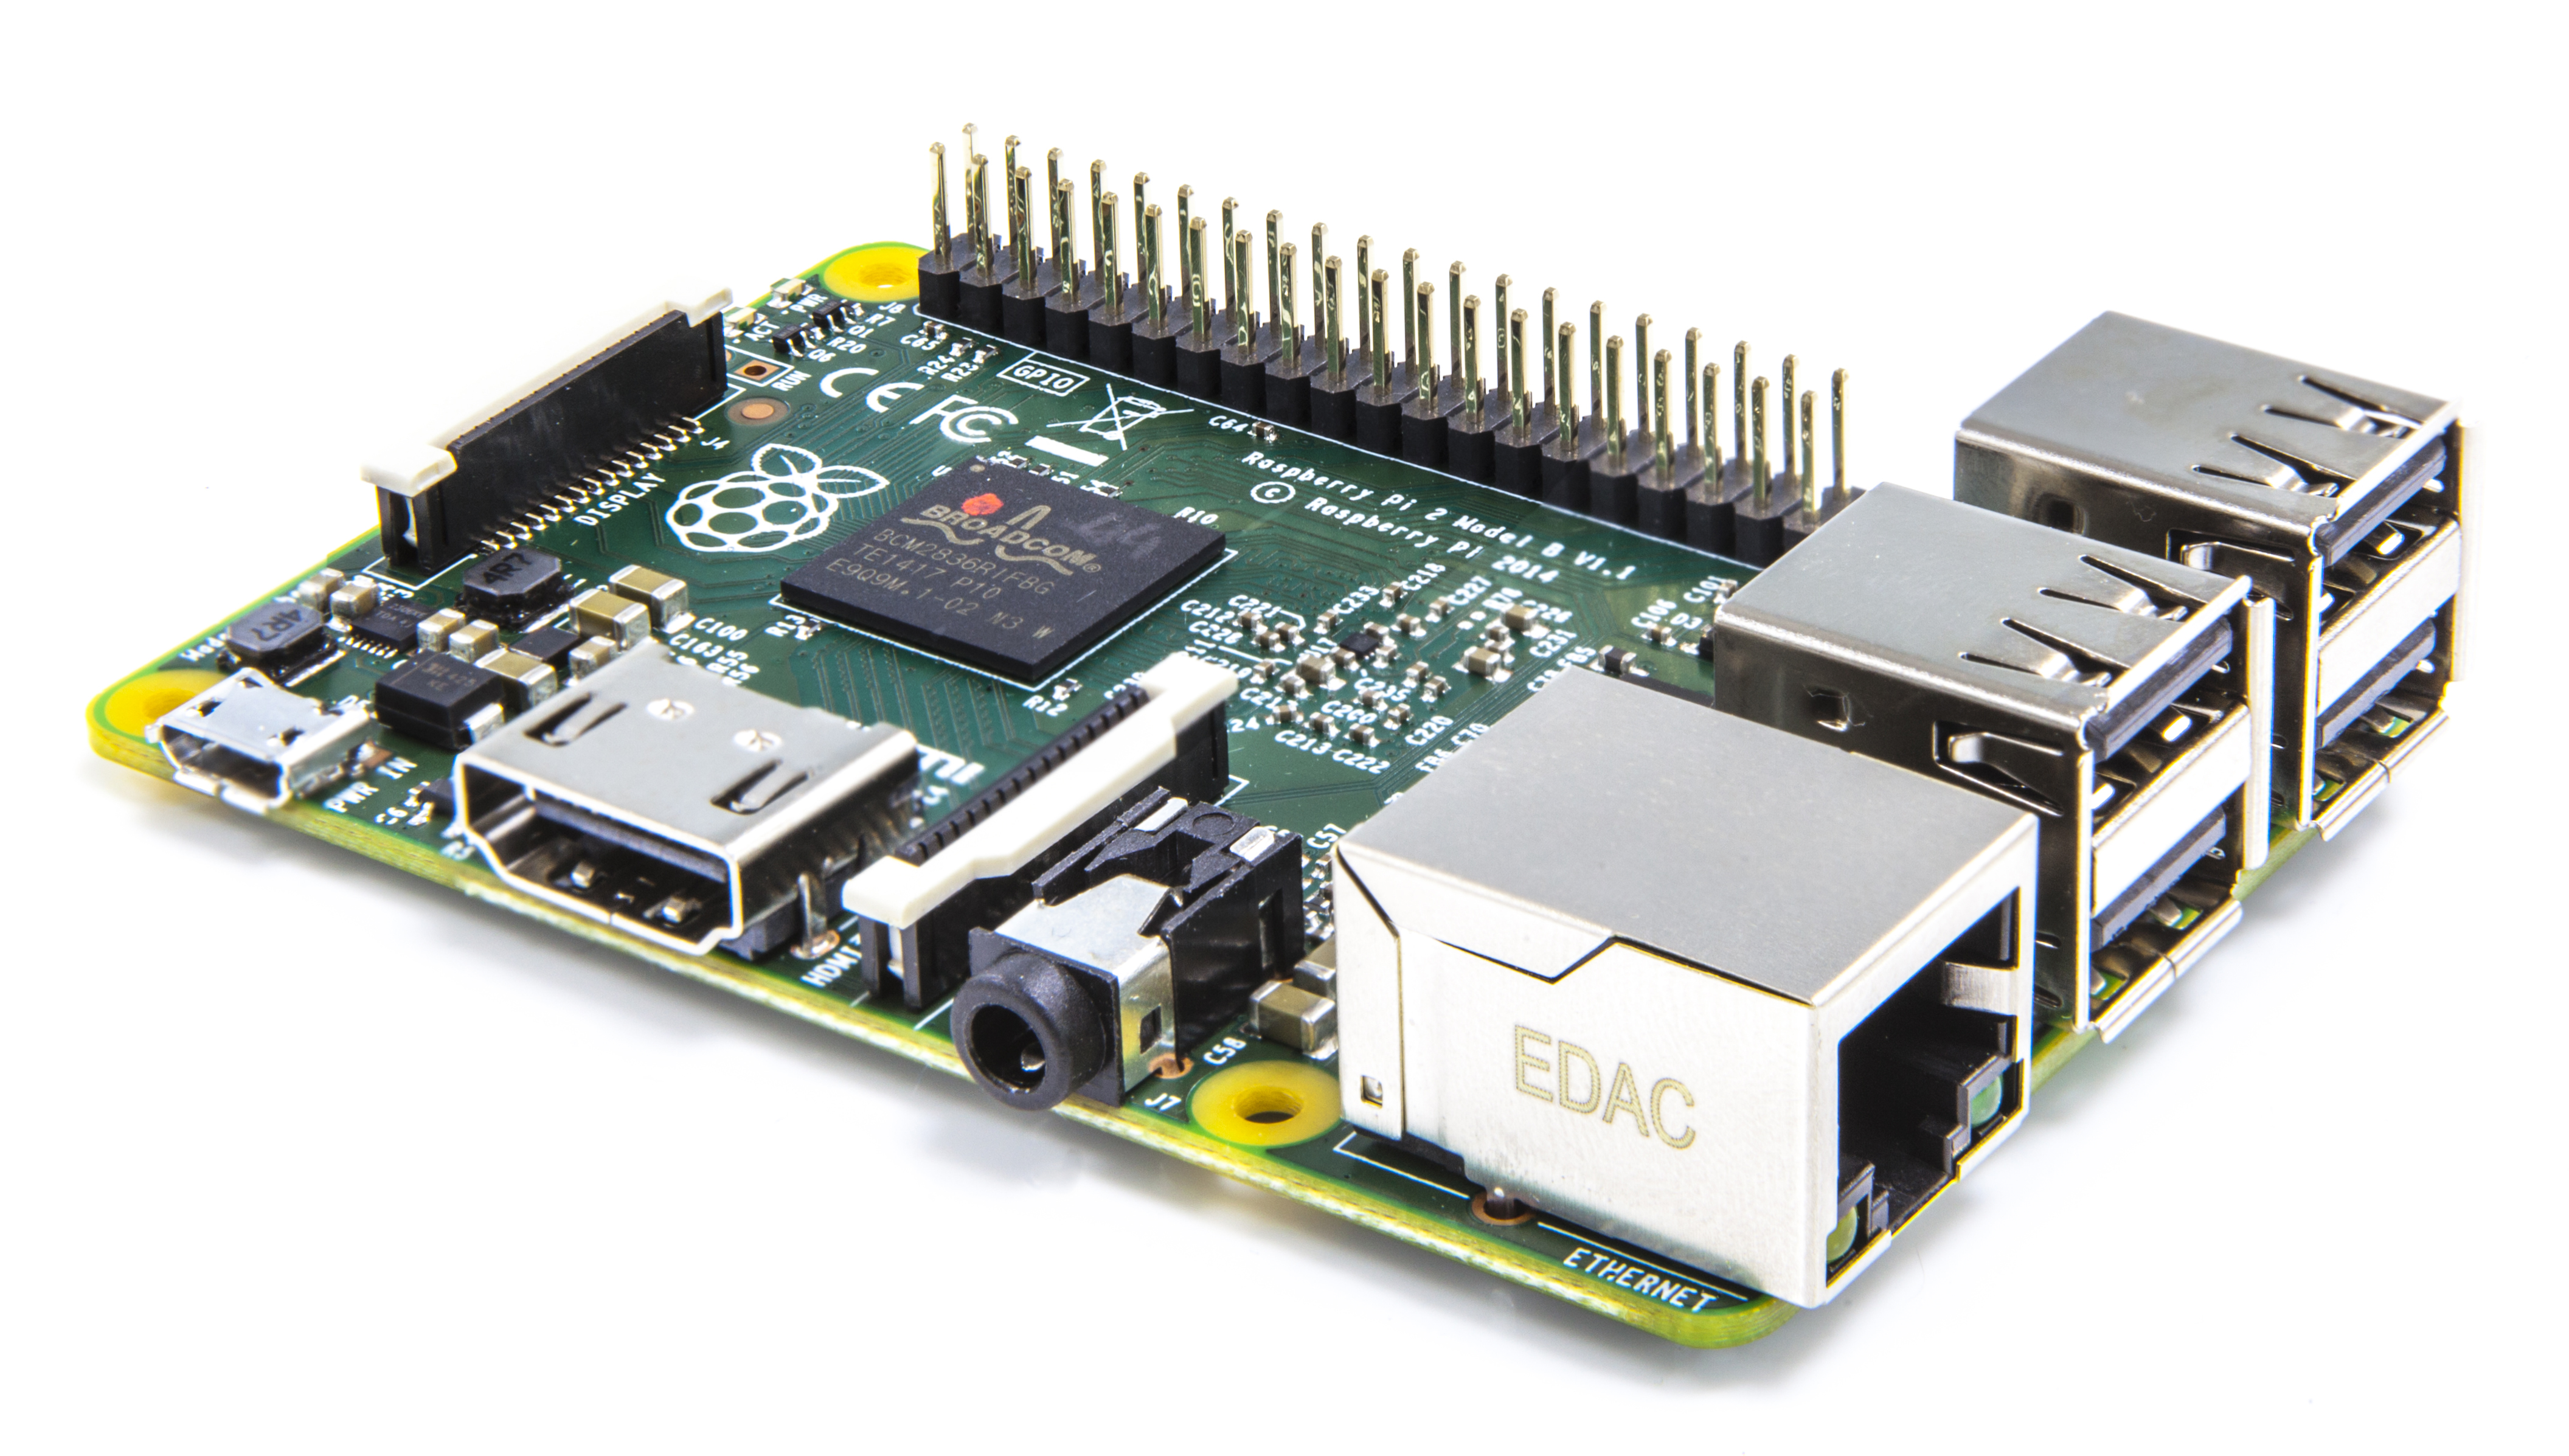
\includegraphics[width=10.0cm]{Pi2.jpg}
\caption{\textit{An image showing Raspberry Pi 2 Model B used for the implementation of the project.}}
\label{fig:Pi2}
\end{figure}
This version of the Pi has the following specifications.
\begin{itemize}
  \item A 900MHz quad-core ARM Cortex-A7 CPU
  \item 1GB RAM
  \item 4 USB ports
  \item 40 GPIO pins
  \item Full HDMI port
  \item Ethernet port
  \item Combined 3.5mm audio jack and composite video
  \item Camera interface (CSI)
  \item Display interface (DSI)
  \item Micro SD card slot
  \item VideoCore IV 3D graphics core
\end{itemize}
\subsection{Raspberry Pi virtualization}
By setting up a virtual Raspberry Pi, the software can be further tested without physically accessing the Raspberry Pi and burning disk images all the time, even after all automatic tests have passed.
Raspberry Pi uses an ARM processor, so the only tool available to emulate it on PCs is \texttt{qemu}.

Basically follow the instructions from \url{http://www.linux-mitterteich.de/fileadmin/datafile/papers/2013/qemu_raspiemu_lug_18_sep_2013.pdf} but use the latest Raspbian image instead, which can be downloaded from \url{https://www.raspberrypi.org/downloads/}.
And download \texttt{kernel-qemu} from \url{http://web.archive.org/web/20150214035104/http://www.xecdesign.com/downloads/linux-qemu/kernel-qemu} because the original page is unavailable.

Currently this solution has several drawbacks, mostly notable ones are low speed and lack of serial port support.

\vspace{\baselineskip}

Note:

\begin{itemize}
\item The second line of \texttt{/etc/udev/rules.d/90-qemu.rules} is indeed \texttt{KERNEL=="sda?", SYMLINK+="mmcblk0p\%n",}, there is a typo in the picture.
\item Although the new RPi 2 model has an ARMv7 processor, Raspbian is still compiled into ARMv6 (for compatibility with old models), so emulating with \texttt{-cpu arm1176} is reasonable.
\end{itemize}

\section{Serial control of the elevator}
\label{sec:Serial_control_of_the_elevator}
The Elevator is controlled by sending a hex encoded signal via serial cable.
In order to move the elevator to floor three, we are sending a signal which is interpreted as a move command to floor three.
One can also send a special "heartbeat" signal that will make the elevator respond with the information about the current floor it is on.
So, when the user enters the elevator cabin and asks to be taken to a certain floor, the user utterance is recognized and the corresponding floor signal is sent.
After the elevator receives the signal it should close the doors and start moving if everything went well.

% we need a few pics here when we finish the setup
%\begin{figure}
%\center{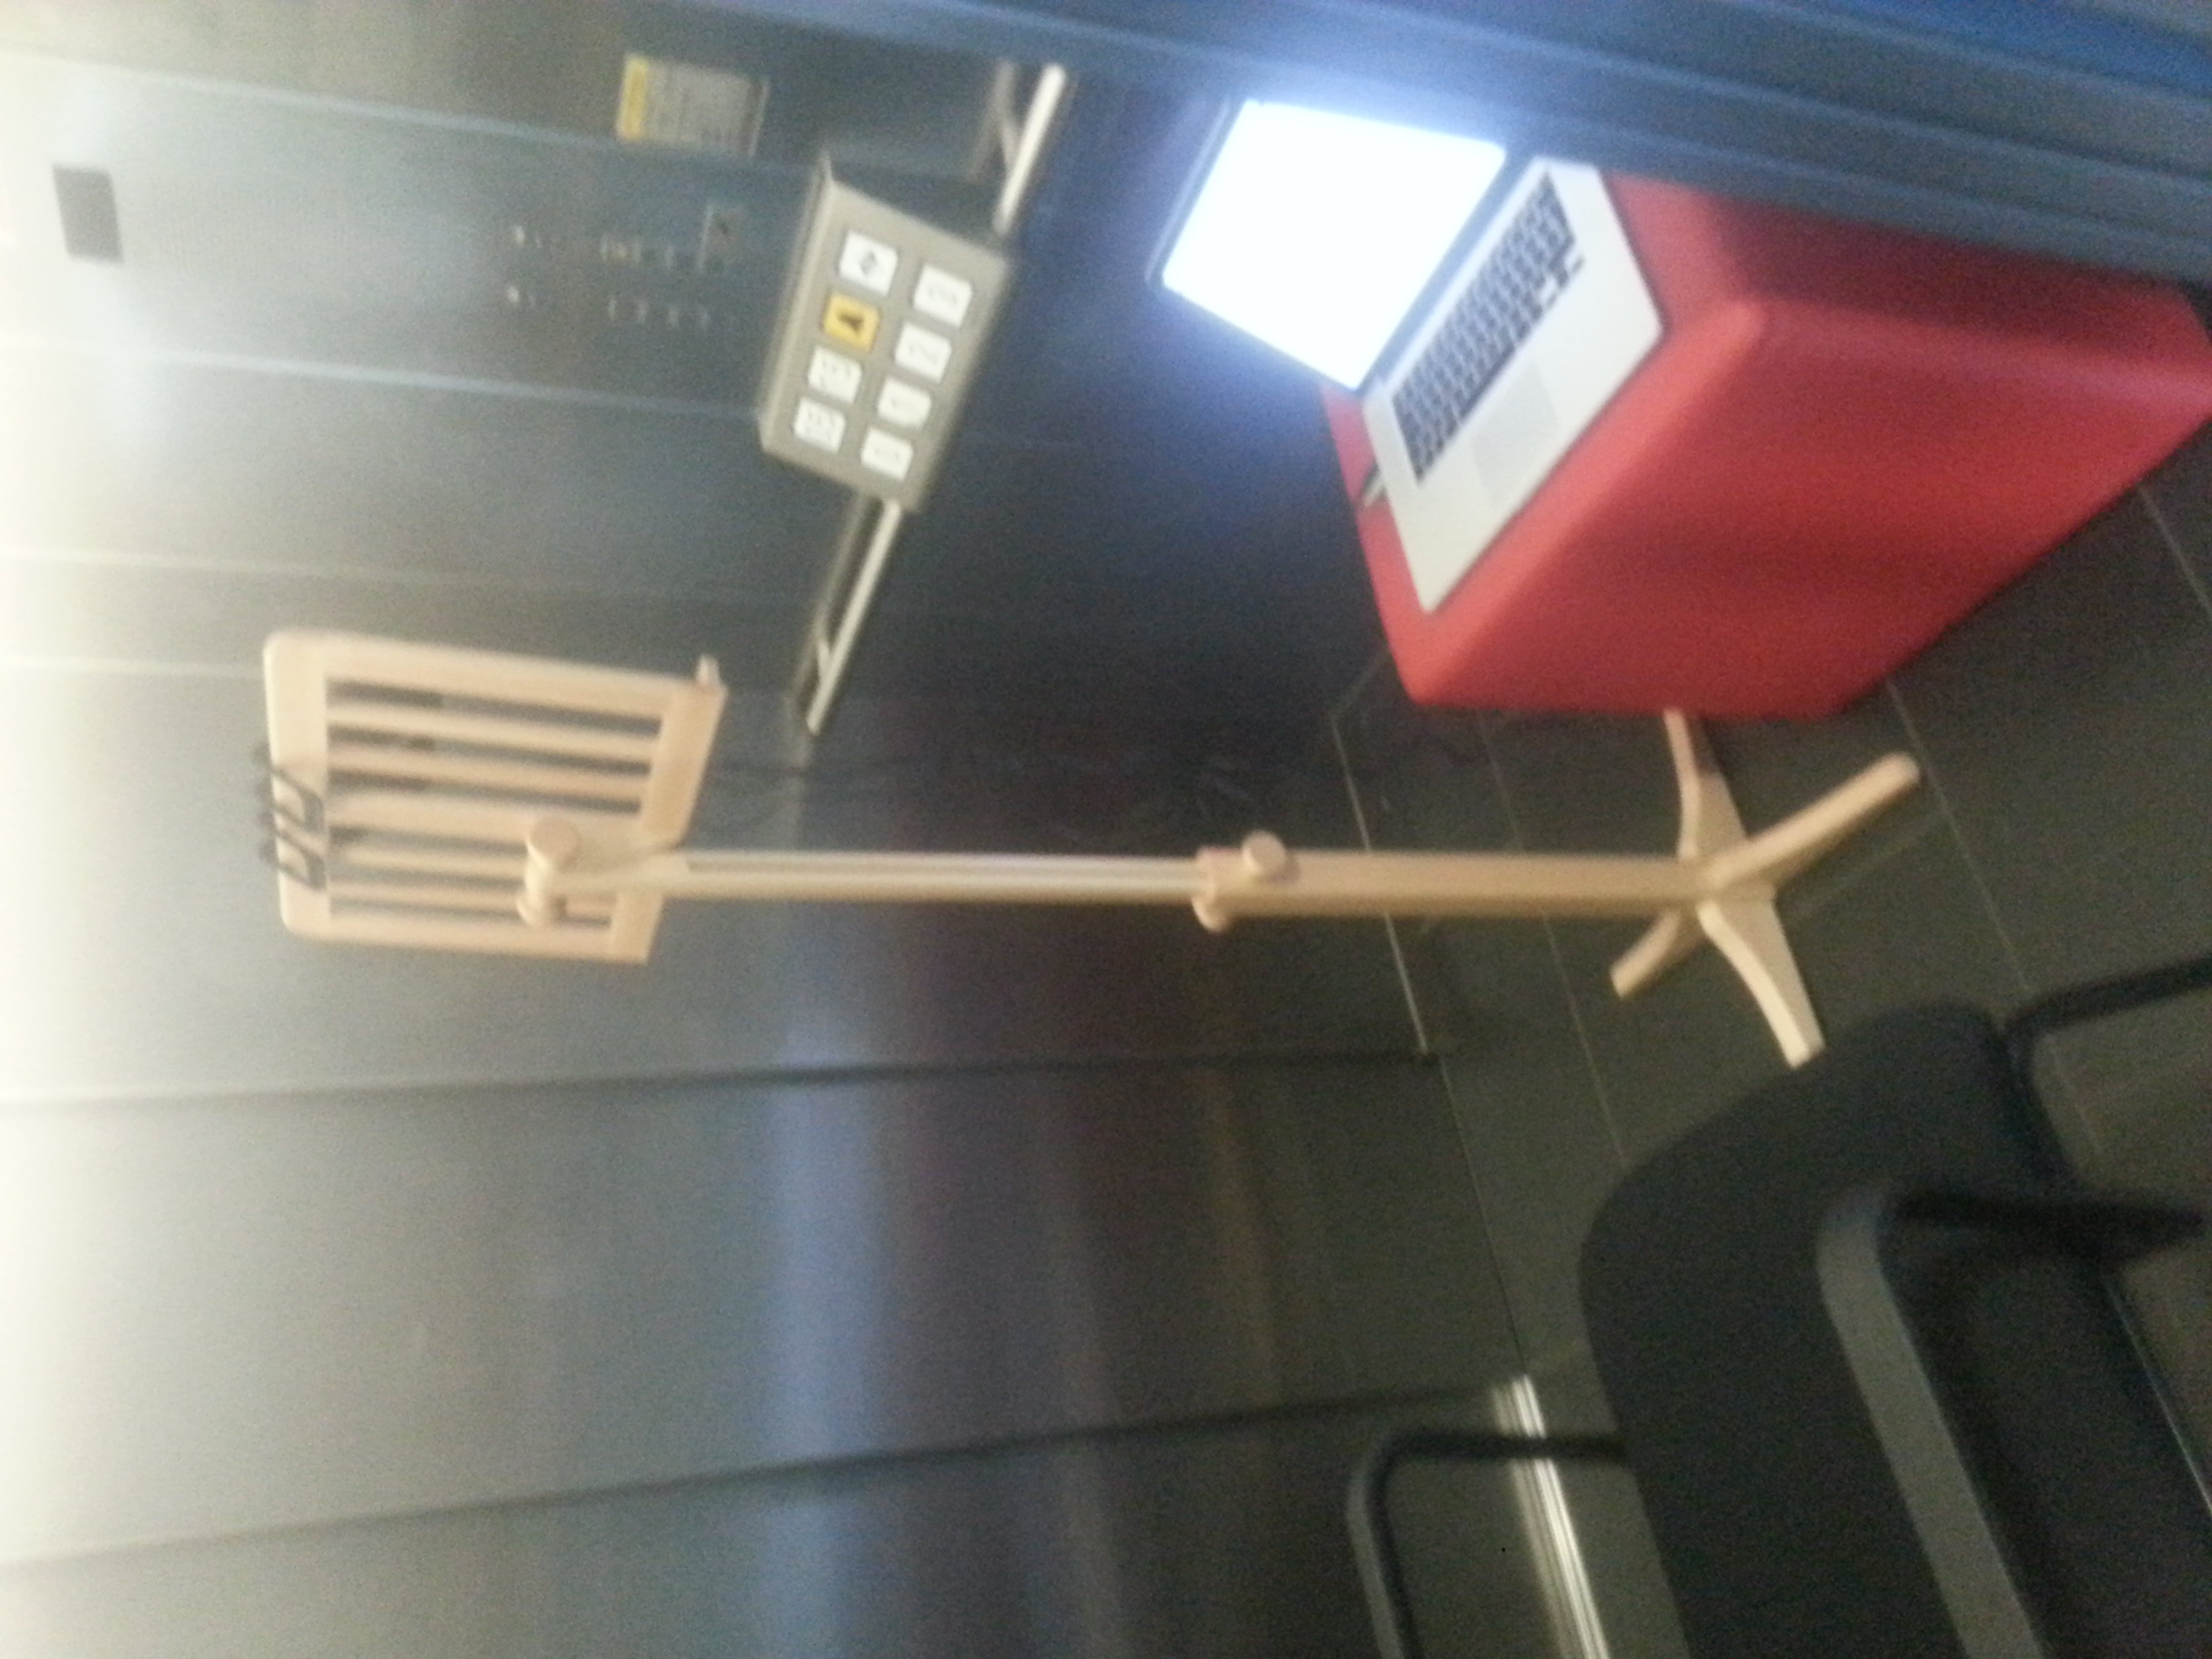
\includegraphics[scale=0.10, angle=-90]{setup_reverberation_rec.jpg}}
%\caption{Recordings setup.}
%\label{fig:recordingsetup}
%\end{figure}

\begin{comment}
\begin{figure}%
\parbox{1.2in}{%
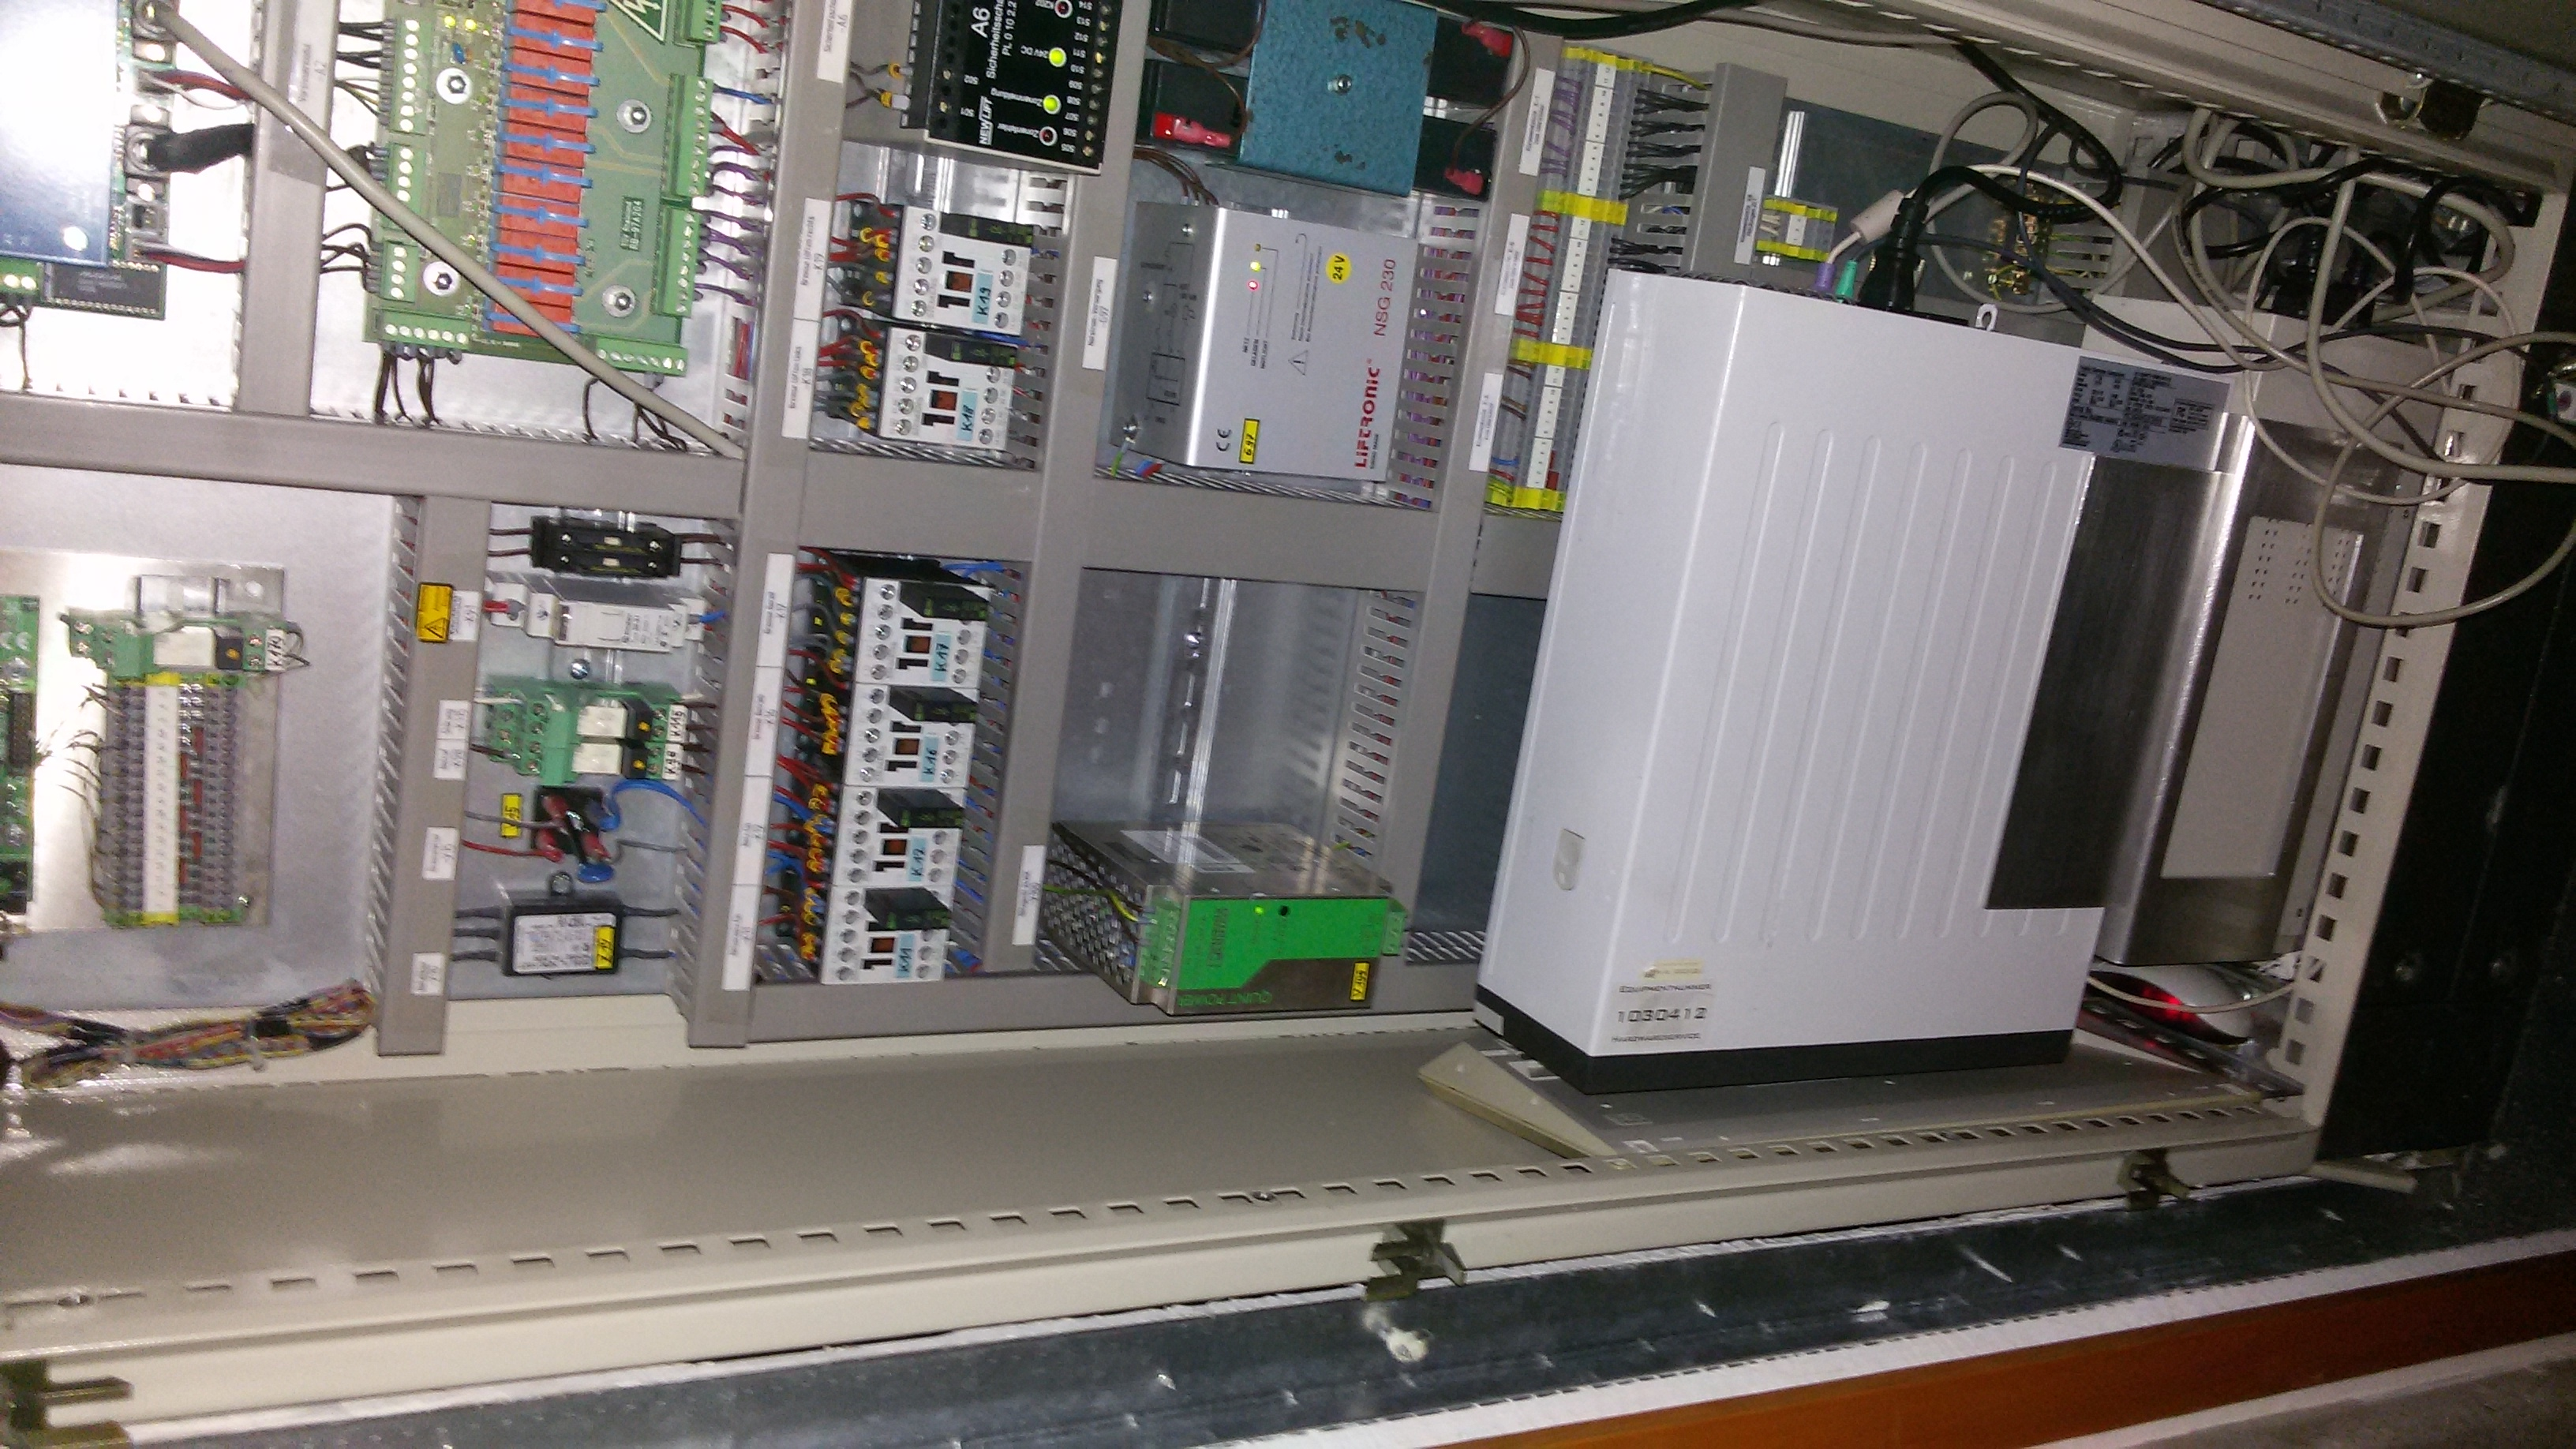
\includegraphics[height=4.0cm, angle=-90]{inside_ellevator1.jpg}
\caption{First.}%
\label{fig:2figsA}}%
\qquad
\hspace{10pt}
\begin{minipage}{1.2in}%
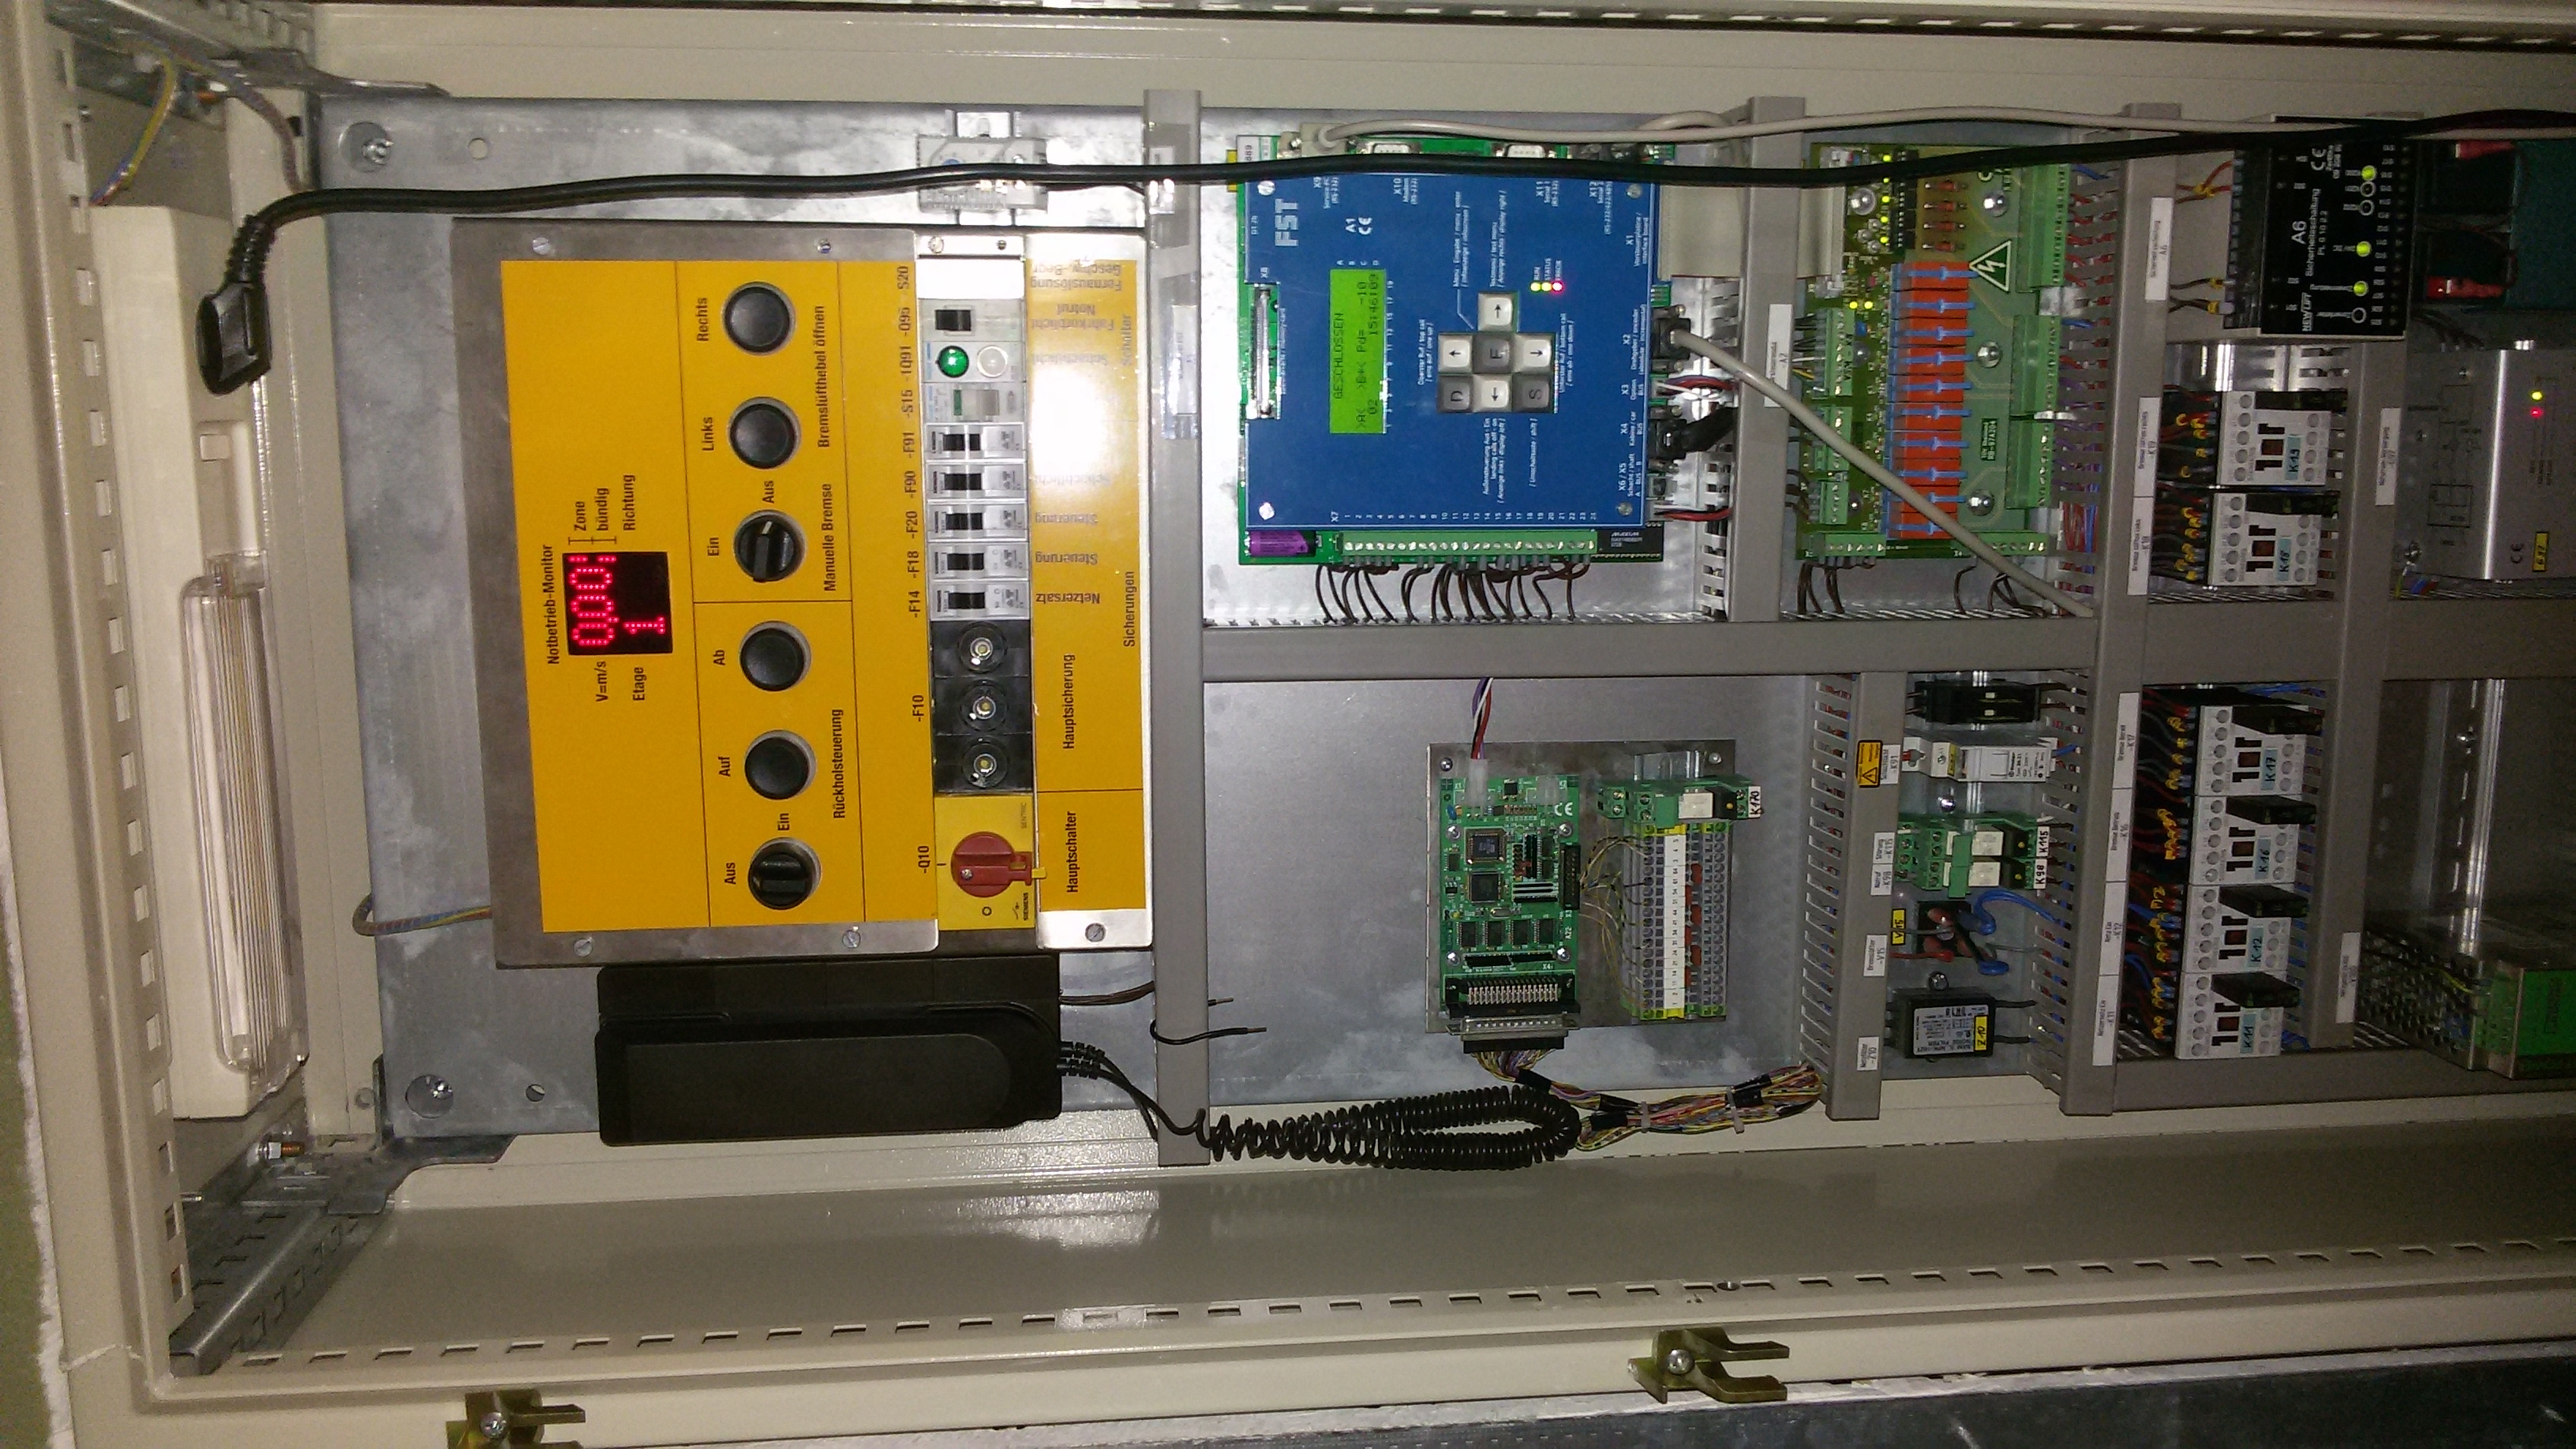
\includegraphics[height=4.0cm, angle=-90]{inside_ellevator3.jpg}
\caption{Second.}%
\label{fig:2figsB}%
\end{minipage}%
\end{figure}%

\begin{figure*}%[t!]
\centering
\begin{subfigure}[b]{0.5\textwidth}
\centering
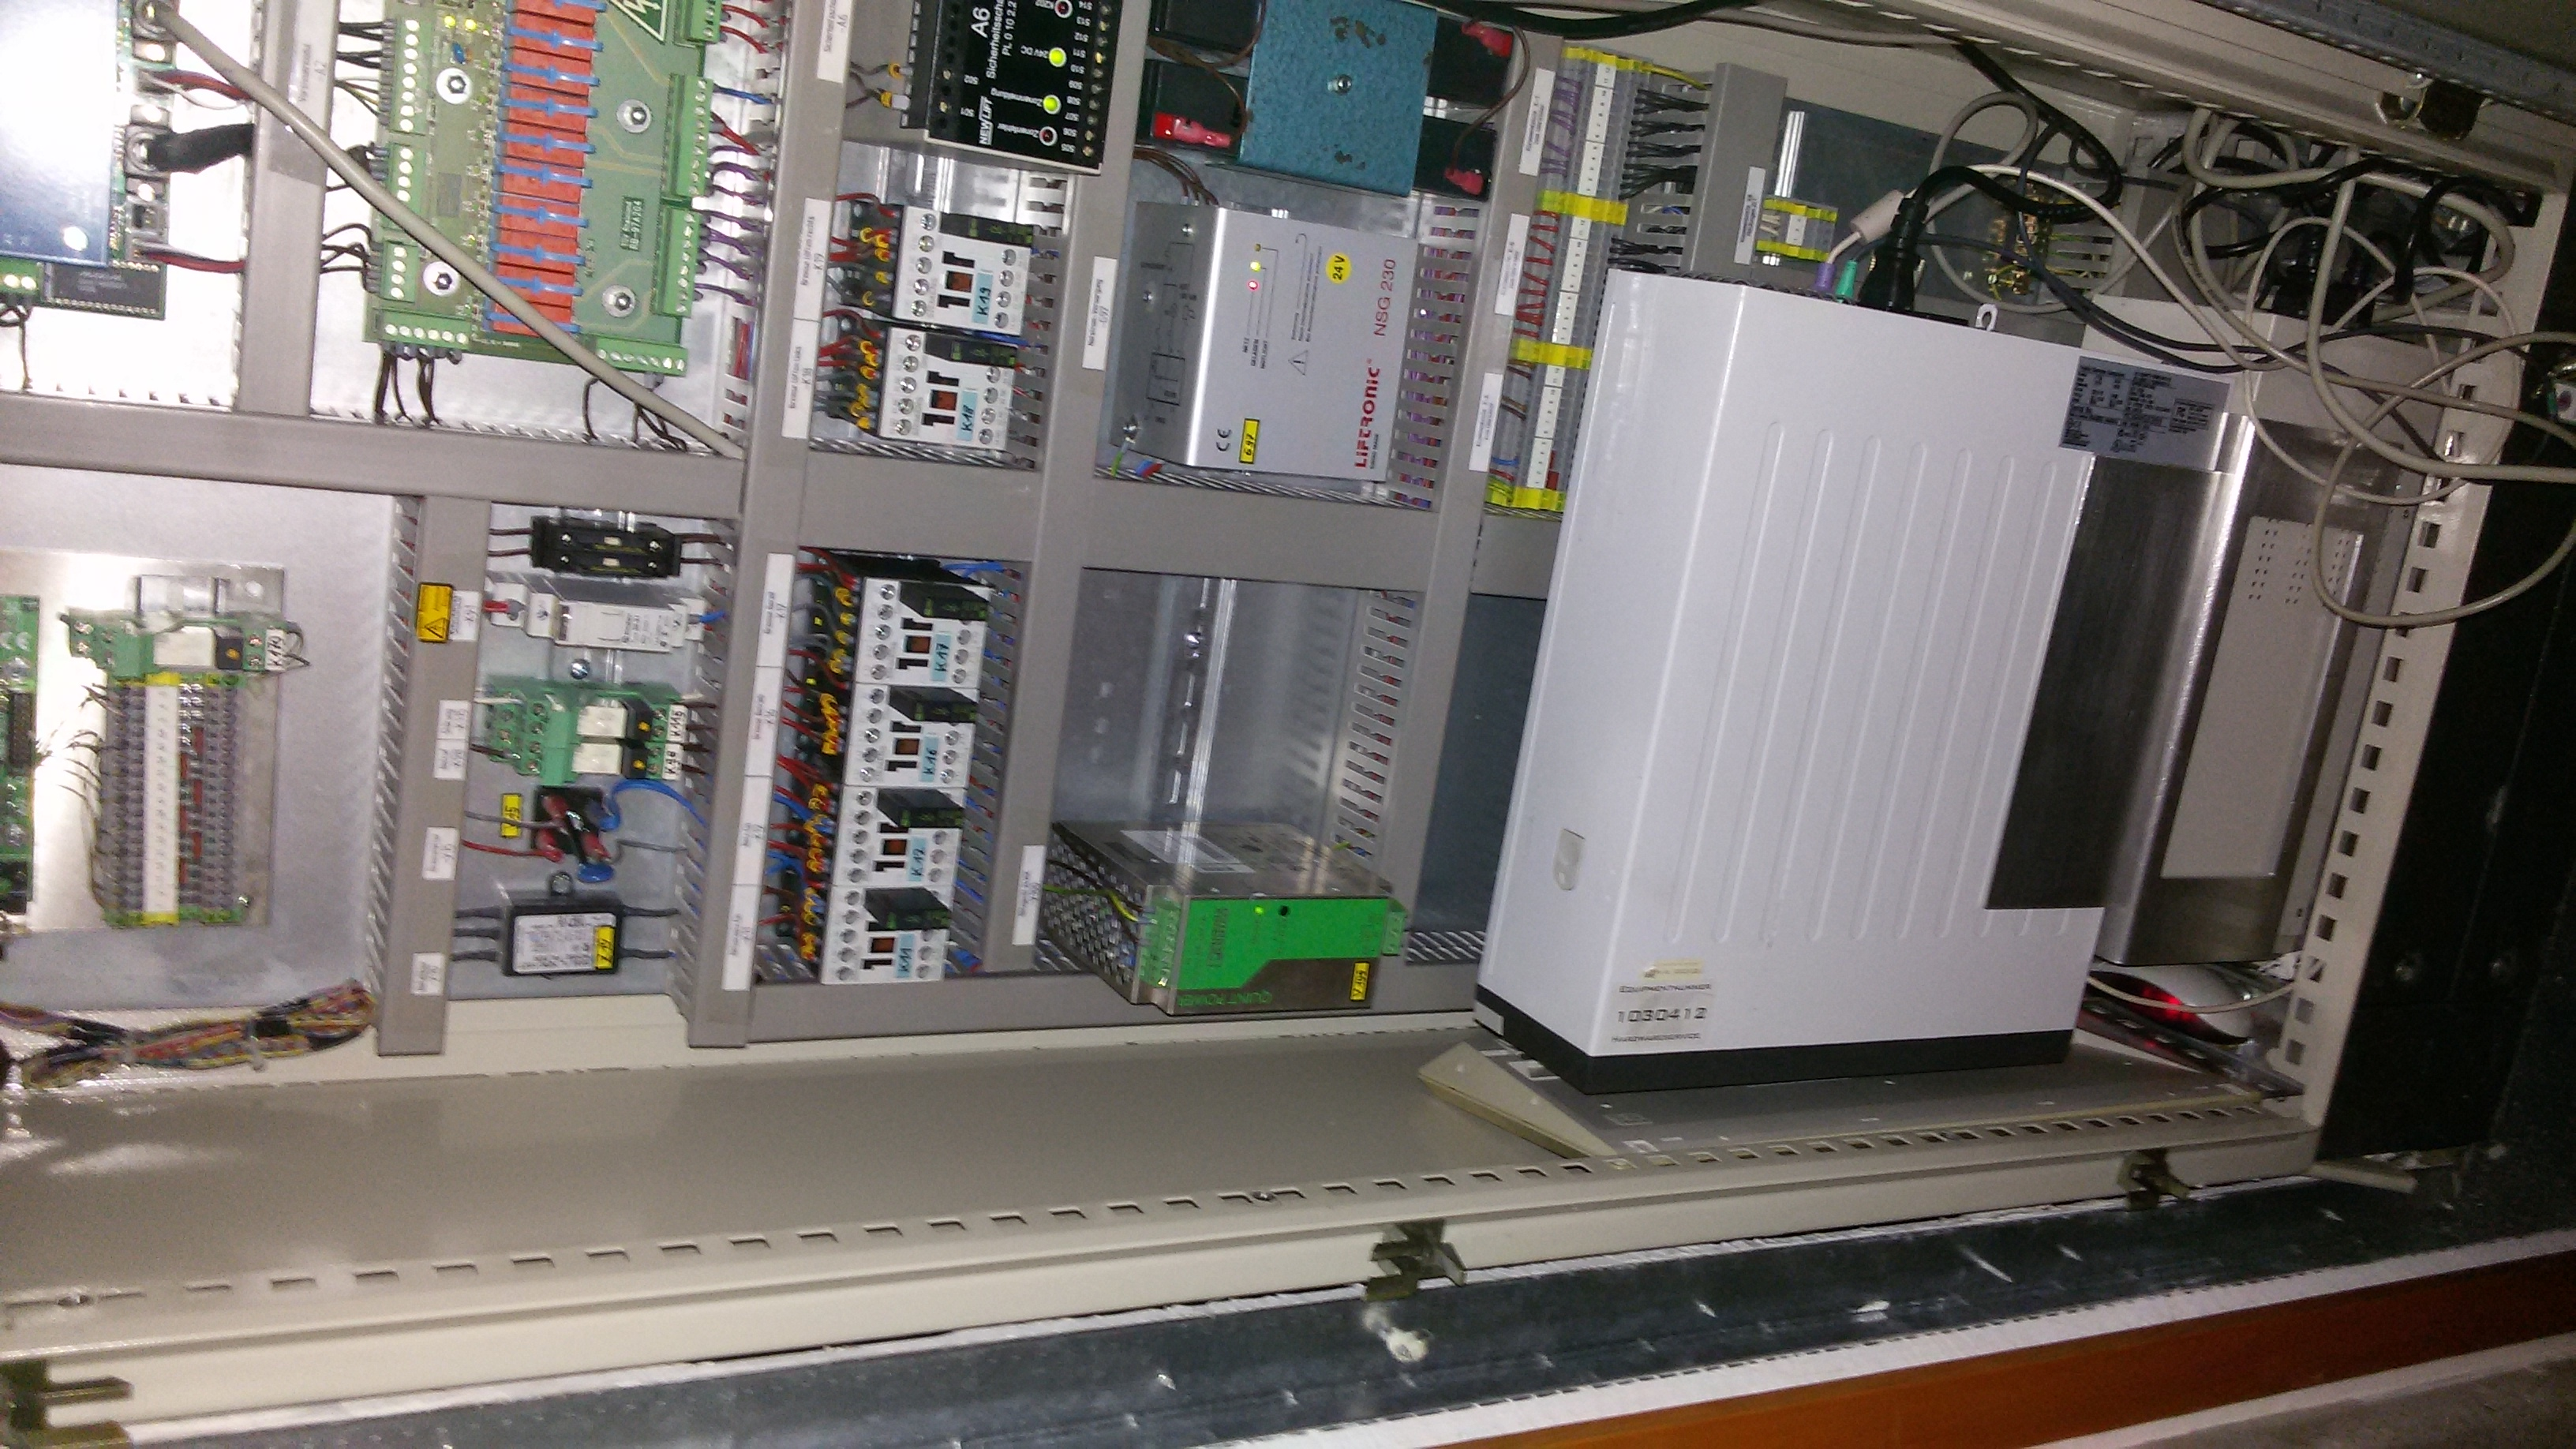
\includegraphics[width=0.5\textwidth, angle=-90]{inside_ellevator1.jpg}
\caption{Lorem ipsum}
\end{subfigure}
~
\begin{subfigure}[b]{0.5\textwidth}
\centering
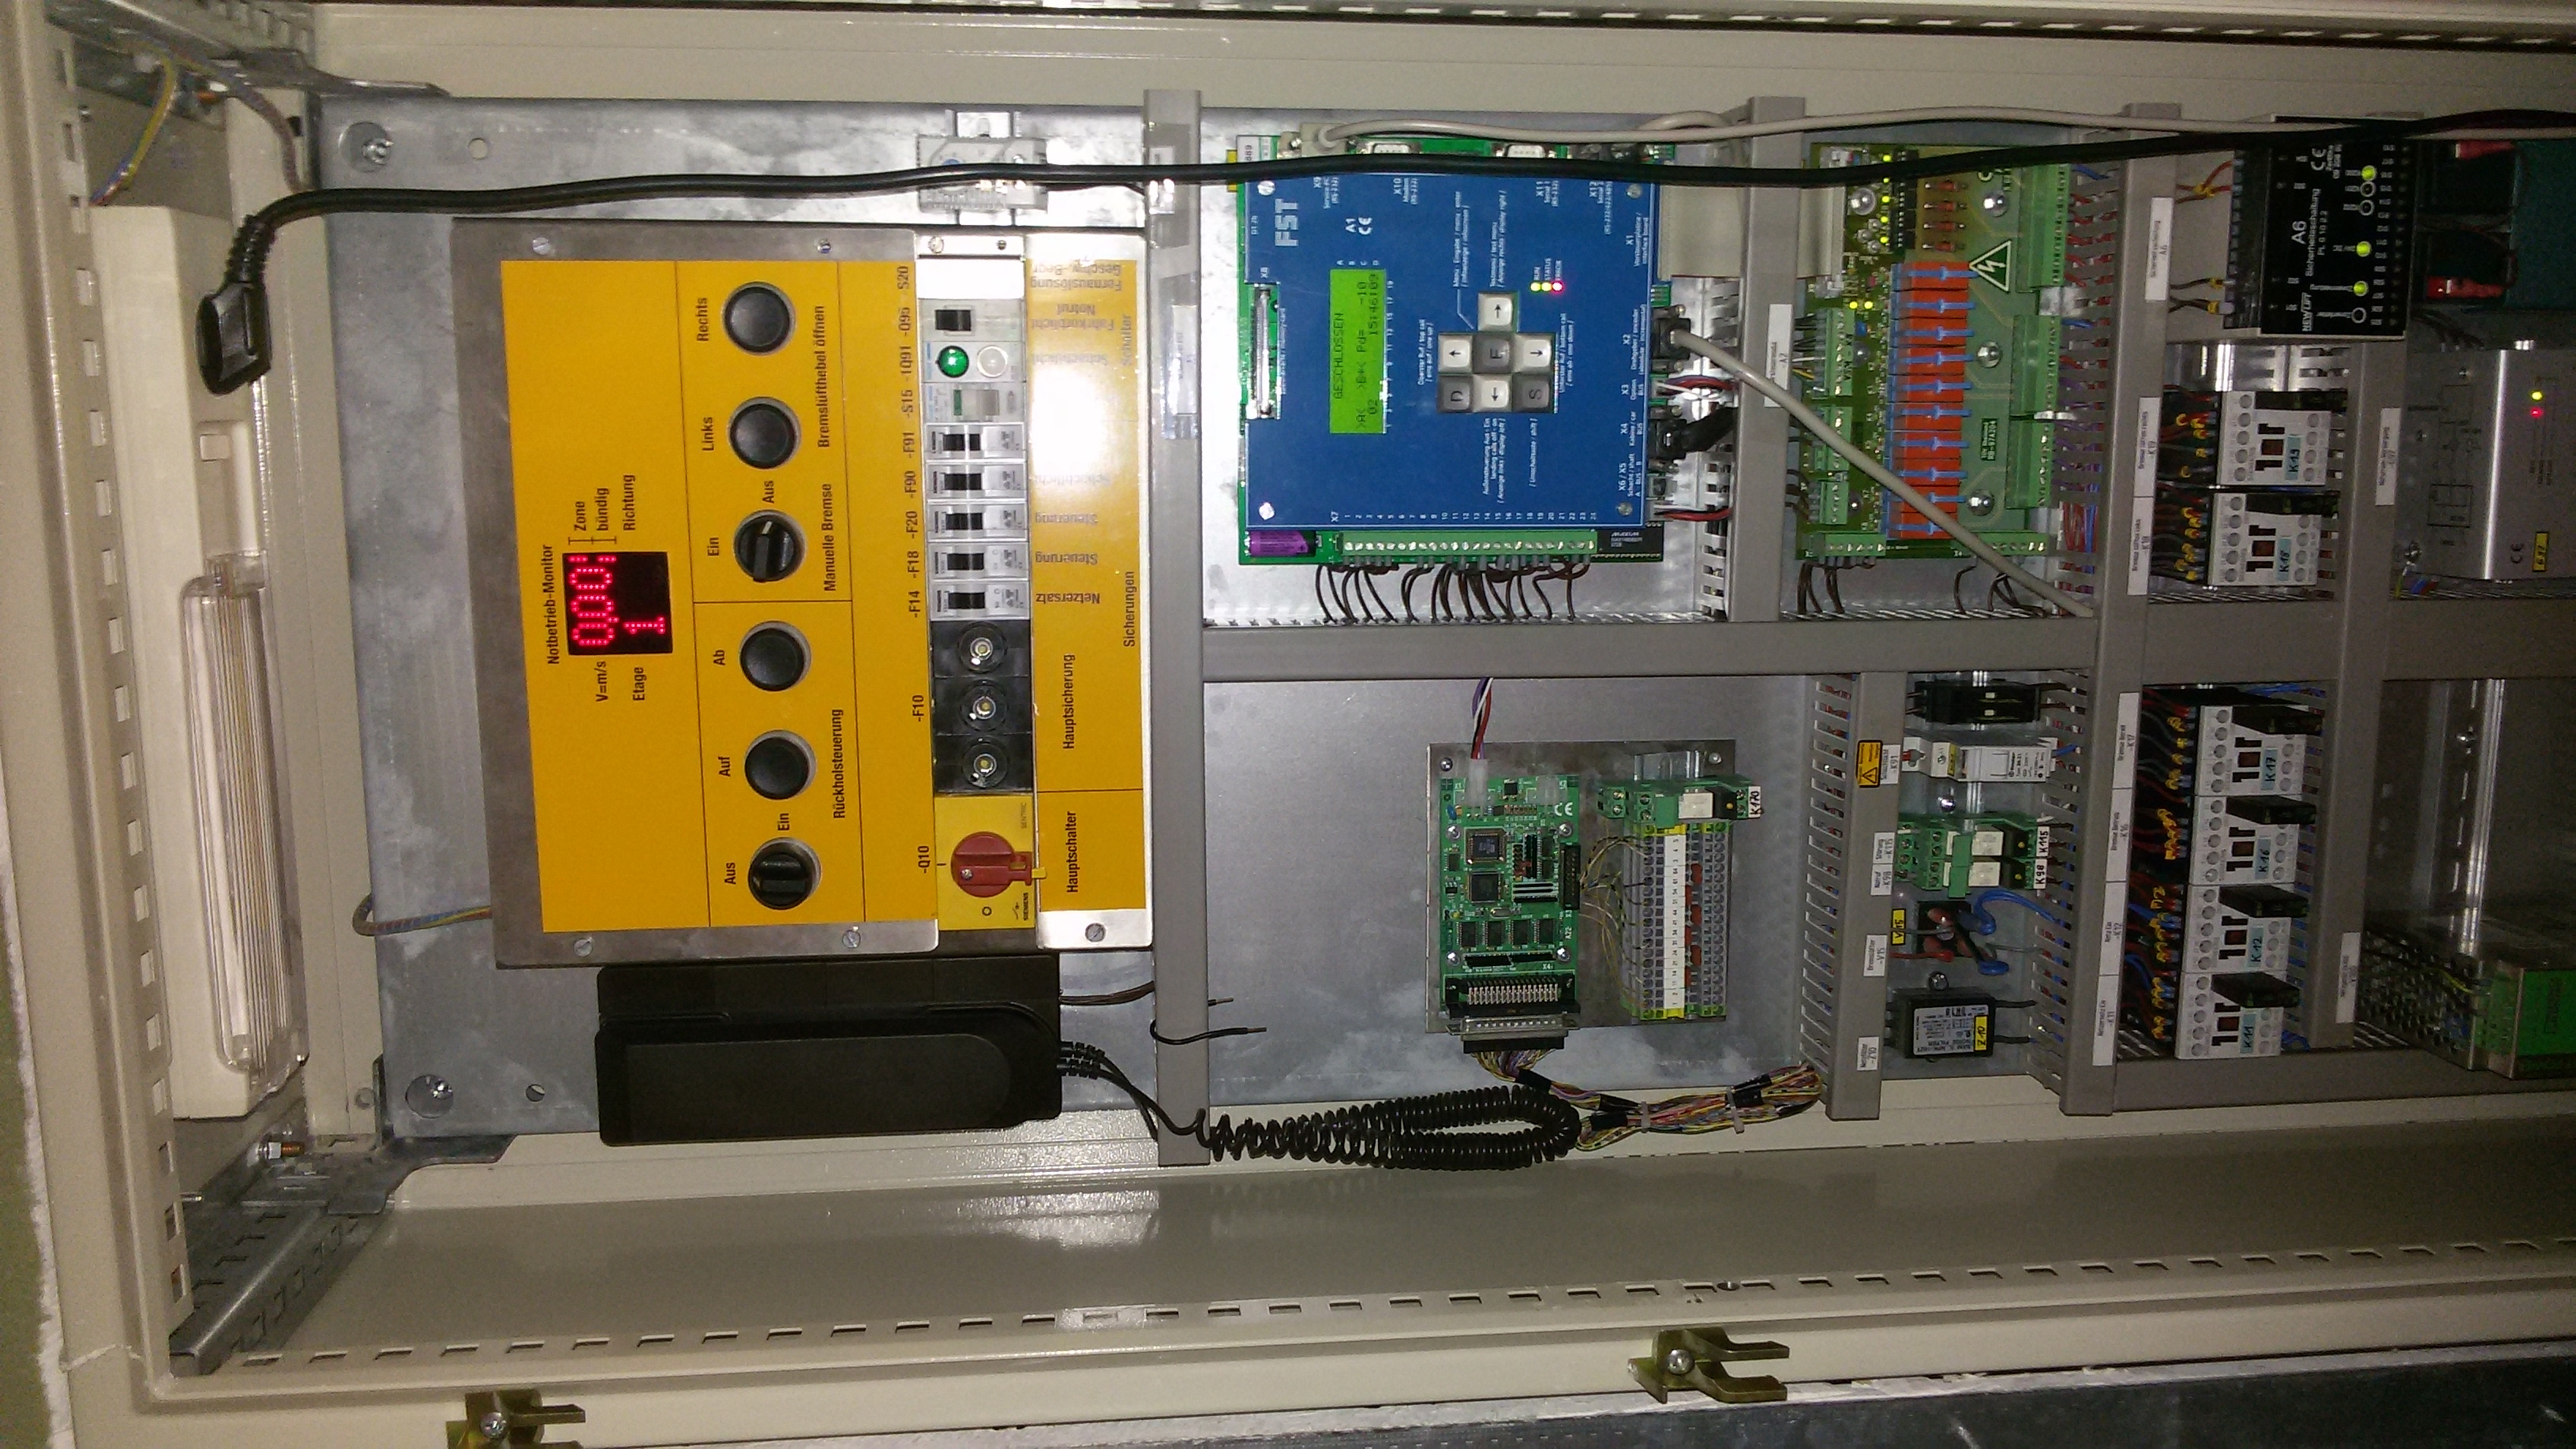
\includegraphics[width=0.5\textwidth, angle=-90]{inside_ellevator3.jpg}
\caption{Lorem ipsum, lorem ipsum,Lorem ipsum, lorem ipsum,Lorem ipsum}
\end{subfigure}
\caption{Caption place holder}
\end{figure*}
\end{comment}

\todo{TODO: a few images of the setup.}
Before working on serial implementation several java libraries for serial communication were reviewed: pi4j, javax.comm, RXTX.
It was decided to stay with RXTX, since pi4j was not stable enough and javax.comm didn't have freely available sources.
Serial implementation follows mainly RXTX examples provided \href{http://rxtx.qbang.org/wiki/index.php/Two_way_communcation_with_the_serial_port}{online} as well as source files of the original project.
For example, floor hex codes and "heartbeat" signal were taken from the original source code.
Several methods from old source files were also used, like the ones that deal with "heartbeat" processing logic.

\subsection{Serial cable connection setup}
\label{sec:Serial_cable_connection_setup}
Raspberry Pi 2 should be connected to the elevator via DE-9 type serial port.
After numerous unsuccessful attempts to connect Raspi to the serial port via its GPIO pins, a USB to serial converter was used.
The new converter worked fine out-of-the-box.
Test signals via serial port from Raspi to desktop PC and vice versa were successfully sent.
After running several tests between Raspi and desktop PC we decided to test serial connection to the elevator.

Signals could be send to the elevator via the serial port, but the elevator was able to move only to one specific floor (0.5 which corresponds to 1 floor).
The signal was interpreted by the elevator as a command to move to floor 1.
This might be due to insufficient power (5V) of Raspi USB to serial connector.
The signal gets garbled upon transmission.
If the serial port power could be boosted up to 12V the connection should stabilize and work correctly.


\subsection{Serial connection implementation}
Within the EllaVator project you can find the following classes that handle serial connection and data transmission between Raspberry Pi and the elevator: \texttt{ElevatorController.java, SerialControllerInterface.java, SerialPortController.java}.\\
\texttt{ElevatorController.java} is basically a wrapper class that instantiates \texttt{SerialPortController} with predefined constant values for serial connection.
These values are important and should not be changed unless you decide to replace Raspberri Pi.\\
Serial port name = \textbf{\texttt{/dev/ttyAMA0}} default serial port on Raspberry Pi.\\
\href{https://en.wikipedia.org/wiki/Serial\_port\#Speed}{Baudrate} = \textbf{38400} proved to work well with our implementation.\\
\href{https://en.wikipedia.org/wiki/Serial\_port\#Data_bits}{Bits} = use \textbf{8} bits.\\
\href{https://en.wikipedia.org/wiki/Serial\_port\#Stop_bits}{Stopbits} = use \textbf{1}.\\
\href{https://en.wikipedia.org/wiki/Serial\_port\#Parity}{Data correction or Parity} = set to \textbf{NO\_PARITY}.\\

All the constants are kept in \texttt{SerialControllerInterface.java} class.
After instantiating \texttt{SerialPortController} the following public methods become available through \texttt{ElevatorController} class: \texttt{getCurrentFloor()} and \texttt{pushButton()}.
Method \texttt{pushButton()} is invoked whenever we want elevator to move to specific floor.
It accepts integers from 0 to 5 where each integer corresponds to specific floor (see \texttt{SerialControllerInterface.java}).
Method \texttt{getCurrentFloor()} should return the integer which represents current floor the elevator is on.
This method triggers \texttt{getReceivedBytes}, \texttt{findValidSubstrings} (taken from original code) and \texttt{checkMessage} (taken from original code).
Method \texttt{findValidSubstrings} triggers \texttt{addByteStringToArrayList}.
Each method is accompanied by extensive information, please read it first.

\subsection{Serail port testing}
It is technically impossible to test Raspi and elevator connection without opening the elevator control panel.
Therefore, an old laptop with serial port and a desktop PC were used.
For testing purposes several python scripts, pi4j java testing tools and a small RXTX java implementation were written.
Shell utilities such as minicom were also used.
\\

There were 3 testing phases.

1 testing:

Python pyserial implementation were used to test serial connection between Raspi, laptop and PC.
After several unsuccessful attempts to use pi4j and GPIO pins connection, the switch was made to a USB serial converter.
Raspi successfully sent the signals via serial port using USB converter.
The serial connection between a laptop and a desktop PC was also tested successfully
Everything worked as expected.
\\

2 testing:

The laptop was connected to the elevator via laptop serial port with a simple serial cord.
Small RXTX serial port utility was used to send the signals from the laptop.
Everything worked correctly and the elevator was controlled from the laptop by sending the appropriate signals.
\\

3 testing:

Raspi was connected to the elevator using USB serial converter.
The same RXTX serial port utility was used to send the signals to the elevator.
However, whatever floor the elevator was sent to, it only ever moved to floor 1.
A reason for this might be that Raspi simply does not have enough power to support serial connection to the elevator.


\newpage
\section{Development tools}
\label{sec:Development_tools}
\subsection{Gradle}
Gradle\footnote{http://gradle.org/} is a build automation tool and simplifies the build process drastically.
Instead of having a readme file that explains how to build the project, building the project is as easy as executing \texttt{./gradlew build} on the command line.

Gradle is configured in the file \texttt{build.gradle}.
Although it looks like a configuration file, it is actually fully functional code written in Groovy\footnote{http://www.groovy-lang.org/}, a scripting language based on Java.

A Gradle wrapper was included in the repository.
This file called \texttt{gradlew} (and \texttt{gradle.bat} for windows) downloads and runs the right Gradle version when executed.
It is recommended to use this file instead of any other locally installed Gradle, because it might be another version of Gradle.

The file \texttt{settings.gradle} specifies the gradle project structure by declaring several subprojects.
There is the opendial subproject, which is a copy of the dialog manager OpenDial\footnote{http://www.opendial-toolkit.net/}.
Next ther is the sphinx4 subproject, consisting of sphinx4-core and sphinx4-data, which is a copy of the speech recognition software Sphinx4~\cite{Walker:2004:SFO:1698193}.
These subprojects are all forked on github from the originals, eventually adapted for the purposes of this project and then included as a git submodule.
Finally there is a subproject called prompts, that is our own making.
It contains example audio prompts for this project, that are used for the acoustic model training and for testing.

\subsection{GitHub}
GitHub is a web platform for collaboration using git, which is a version control system.
This system was used to allow several people work on the same project at the same time without overwriting each others changes.

For some of the dependencies (Sphinx, OpenDial) git submodules were used to include them into the project.
This allows to adapt the original code for purposes of this project if necessary.
In order to download these dependencies when you clone the repository, you must therefore execute
\begin{lstlisting}[language=bash]
git clone https://github.com/EllaVator/EllaVator.git --recursive
\end{lstlisting}
or init and update all of the subprojects individually.
\subsection{Continuous integration with Travis CI}

Continuous integration is based on the idea that all developers send their changes to a common code repository as soon as possible, for example on GitHub like in this project.
Additionally these changes should be tested before they are merged into the main code repository.
In order to do this automatically, it is necessary to automate the build process completely, as was done in this project  using Gradle.
If the build succeeds, all unit and integration tests can be executed, which prevents non-working code to enter the main repository if the error is covered by a test case.
This procedure is much better than having each developer running the tests before committing the changes to the main repository for a couple of reasons.
Firstly, it does not rely on the developer to run all the tests which can be easily forgotten or skipped, because the developer does not see the whole effect his modification has.
Secondly, the project is built in a “neutral” environment that should be a close copy of the production environment if possible.
For example, code that runs fine on the developer's Windows machine but not on Linux can be detected this way.

As it integrates seamlessly into GitHub, Travis CI was used as continuous integration service in this project.
Each pull request gets marked by colors: yellow means the build is still running, red means failed build or failed test, green says everything is OK.
In each pull request there is a link to Travis that gives details about the build process, too.

Travis is configured by a file named \texttt{.travis.yml} in the root directory of the project.
It is not even necessary to specify that the build process is handled by Gradle.
Travis can detect this automatically, given that groovy is specified as project language (\texttt{language: groovy}).
Java 8 had to be used, because this is a minimum requirement for Opendial.
Also, Travis must install the \texttt{sox} command, which is used to extract single sentences from the test audio files in the prompts subproject.
Finally, the gradle files are cached to speed up the build process (otherwise the Gradle wrapper will download Gradle every time).

Each developer can add Travis to his own repositories, too.
That way failures can be detected even before sending a pull request.
Travis can be activated by signing up on \url{https://travis-ci.org/} using your GitHub account.
Then go to your profile page on Travis and activate the GitHub repositories you want to be watched (which must contain a \texttt{.travis.yml} file).
From then on every push to these repositories will trigger Travis to build and run tests and send an email about the result.

\newpage
\section{Testing}
\label{sec:Testing}
Software testing is an essential process in modern software development, in particular in the process of quality assurance (QA) of software.
Generally there at least two types of tests: unit and integration tests.
While unit tests are thought to test small components (e.g. classes) in isolation, integration tests verify how these components work as a whole.

Seeing time constraints and also lack of experience, the decision was made not to be as strict with testing, and to put a focus on integration testing.
All tests are placed in the \texttt{test} source set, i.e. under \texttt{src/test}.
There they can be found automatically by gradle when executing \texttt{./gradlew test} in the commandline.
TestNG\footnote{http://testng.org/doc/} was used as testing framework in this project.

As an example let us have a look at the test called \texttt{SpeechIOTest} in \texttt{src/test/groovy}.

The package relevant for testing is imported like this:
\begin{lstlisting}[language=java]
import org.testng.annotations.*
\end{lstlisting}
Annotations are markers for methods (and other language elements), that start with an @ sign.
For instance, you can see the \texttt{@Test} annotation in line 31.
This marks the following method as a test method which means that this method is called when the tests are run by TestNG or indirectly by gradle.
Usually these test methods also contain one or more \texttt{assert} statements like in this example:
\begin{lstlisting}[language=java]
assert actual == expected
\end{lstlisting}
Asserting something means that the test will only succeed if the condition evaluates to true.
Here the test asserts that the string that was recognized by the ASR from an audio file is identical with the words that actually were spoken in that file.

In this case there is the additional parameter \texttt{dataProvider = 'expandedGrammar'} in the \texttt{@Test} annotation.
This indicates that the test has to be executed multiple times with different test data, which is a very useful feature of TestNG.
The string \texttt{expandedGrammar} refers to the method of this name, that will return the test data as an array.
Each item in this array is an array of parameters that will be passed to the test function.

\newpage
\section{Installation instructions}
\label{sec:Installation_instructions}
These installation instructions have been tested on Ubuntu 14.04.

If you have not installed git on your system, you should do this first:
\begin{lstlisting}[language=bash]
sudo apt-get install git
\end{lstlisting}

This program is the version control system used in this project and helps to keep changes by different developers in sync.
For details see the section on Github.

Now you can download the project files using the \texttt{git clone} command.
Navigate to the folder where you want to place the project files and execute:
\begin{lstlisting}[language=bash]
git clone https://github.com/EllaVator/EllaVator.git --recursive
\end{lstlisting}

This will create a folder named \texttt{EllaVator} inside the current directory and put the downloaded files inside.
Please note that you should use the \texttt{--recursive} flag here in order to download all the nessecary files, including the subprojects.

Now enter the created folder:
\begin{lstlisting}[language=bash]
cd EllaVator
\end{lstlisting}

This project requires Java 8. If you haven't installed it already, you can do so using the following commands:
\begin{lstlisting}[language=bash]
sudo add-apt-repository ppa:webupd8team/java
sudo apt-get update
sudo apt-get install oracle-java8-installer
\end{lstlisting}

Now you can build or run the project using one of the following commands:
\begin{lstlisting}[language=bash]
./gradlew build
./gradlew run
\end{lstlisting}

\cleardoublepage
\begin{appendix}
\section{Recorded sentences} \label{prompts}
\subsection{English elevator commands}
\begin{itemize}
\item To the eye-tracking experiment
\item I would like to go up
\item To office three seventeen
\item To the restroom
\item To the reading laboratory please
\item Please to the ground level
\item Third floor thank you
\item To the conference room
\item To the aquarium
\item Down thank you
\item Office one seventeen thank you
\item Room three hundred and twelve please
\item I would like to go to the office two zero four
\item Room two hundred and two
\item I would like to go to the top floor
\item Vera Demberg's office
\item Please Manfred Pinkal's room
\item Hello
\item To the guest kitchen
\item To the first floor
\item To the mezzanine
\item To room oh oh seven
\item To Maria's office
\item To Dr. Steiner's office
\item Skywards
\item Tell me how to get to the lab.
\item Where is the restroom?
\item Open.
\item Close doors.
\item Hurry up.
\item Bring me to double oh four, please.
\item I would like to see Maria Staudte.
\item Where is Ross Macdonald's office?
\item Which floor is Arif Khan's room?
\item Room one point one.
\item To the top floor.
\item Bring me to where Alexander Hewer's office is.
\item Can you tell me where Hongxia Shi's office is?
\item Can you lift me up to floor two, please?
\item Two floors up please.
\end{itemize}



\subsection{German elevator commands}
\begin{itemize}
\item Bring mich bitte zu null null eins.
\item Ich möchte zu Maria Staudte.
\item Wo ist Ross Macdonalds Büro?
\item In welcher Etage arbeitet Arif Khan?
\item Raum eins punkt eins.
\item Bis ganz nach oben.
\item Bringe mich in den Stock, in dem Alexander Hewers Büro ist.
\item Wo ist denn Hongxia Shis Büro?
\item Kannst du mich bitte in die zweite Etage bringen?
\item Zwei Stockwerke höher bitte.
\item Ich suche das Eye-Tracking Labor.
\item Zum Labor bitte.
\item Zum Aufnahmestudio bitte.
\item Ich muss zur Gästeküche.
\item Zum Aquarium.
\item Zum Büro dreihundertundachtzehn.
\item Zur Toilette bitte.
\item Ich möchte das Gebäude verlassen.
\item Ich suche das Lese-Experiment.
\item Ich habe es eilig.
\item Zum Konferenzraum.
\item Ins dritte Stockwerk.
\item Ins zweite Sockwerk.
\item Ins erste Stockwerk.
\item Einmal nach unten bitte.
\item Zu Professor Pinkal.
\item Zur Gruppe von Dr. Demberg.
\end{itemize}


\subsection{Harvard sentences}
\begin{itemize}
\item The birch canoe slid on the smooth planks.
\item Glue the sheet to the dark blue background.
\item It's easy to tell the depth of a well.
\item These days a chicken leg is a rare dish.
\item Rice is often served in round bowls.
\item The juice of lemons makes fine punch.
\item The box was thrown beside the parked truck.
\item The hogs were fed chopped corn and garbage.
\item Four hours of steady work faced us.
\item Large size in stockings is hard to sell.
\item The boy was there when the sun rose.
\item A rod is used to catch pink salmon.
\item The source of the huge river is the clear spring.
\item Kick the ball straight and follow through.
\item Help the woman get back to her feet.
\item A pot of tea helps to pass the evening.
\item Smoky fires lack flame and heat.
\item The soft cushion broke the man's fall.
\item The salt breeze came across from the sea.
\item The girl at the booth sold fifty bonds.
\end{itemize}


\subsection{Sentences from BITS}
\begin{itemize}
\item Das Dunkel war ein kurzes und leiser werdendes Verschwinden.
\item Er sah sich im Karstadt-Kaufhaus um
\item Fahr, hat er gesagt, um das Hindernis herum.
\item Gemütlicher Abend auf der Weser mit Kohlfahrt ab Martini-Anleger
\item Das Schiff wogte auf den starken Wellen hin und her.
\item Der schnellste Weg zum Jenseits führt kopfüber in die Nacht.
\item Zu schade für's Altpapier.
\item Zu den Ressorts Arbeit und Frauen könnte noch Gesundheit oder Soziales hinzukommen.
\item Weltausstellung in Hannover ökologisch vertretbar.
\item Das Gemälde ohne Titel in Tusche auf Papier.
\item In Ungarn zeigt die Abbildung eine Zahnbürste mit Zahnpasta.
\item Ein Computer besitzt im Allgemeinen Prozessor, Arbeitsspeicher und Festplatte.
\item Das Netzwerk hilft dem Automotor auf das Motorrad.
\item Die Telekom drückt mit ihrer Preispolitik kräftig auf das Bremspedal.
\item Der Lehrer benutzte den Projektor im Unterricht.
\item In der Linguistik kommt es zu Meinungsverschiedenheiten zwischen Fundis und Realos.
\item Die Sprache ist ein weltweites Medium der Kommunikation.
\item Hervor trat ein langes Messer im Suhrkamp-Verlag
\item Wo Wilhelm Busch zur Schule ging.
\item Unter anderem flog Lufthansa von Friedrichshafen nach Oldenburg.
\end{itemize}
\end{appendix}

\cleardoublepage
\bibliography{final_doc}
\bibliographystyle{unsrt}


\end{document}
